%%% Hlavní soubor. Zde se definují základní parametry a odkazuje se na ostatní části. %%%

%% Verze pro jednostranný tisk:
% Okraje: levý 40mm, pravý 25mm, horní a dolní 25mm
% (ale pozor, LaTeX si sám přidává 1in)
\documentclass[12pt,a4paper]{report}
\setlength\textwidth{145mm}
\setlength\textheight{247mm}
\setlength\oddsidemargin{15mm}
\setlength\evensidemargin{15mm}
\setlength\topmargin{0mm}
\setlength\headsep{0mm}
\setlength\headheight{0mm}
% \openright zařídí, aby následující text začínal na pravé straně knihy
\let\openright=\clearpage

%% Vytváříme PDF/A-2u
\usepackage[a-2u]{pdfx}

%% Přepneme na českou sazbu a fonty Latin Modern
\usepackage[czech]{babel}
\usepackage{lmodern}
\usepackage[T1]{fontenc}
\usepackage{textcomp}

%% Použité kódování znaků: obvykle latin2, cp1250 nebo utf8:
\usepackage[utf8]{inputenc}

%%% Další užitečné balíčky (jsou součástí běžných distribucí LaTeXu)
\usepackage{amsmath}        % rozšíření pro sazbu matematiky
\usepackage{amsfonts}       % matematické fonty
\usepackage{amsthm}         % sazba vět, definic apod.
\usepackage{bbding}         % balíček s nejrůznějšími symboly
			    % (čtverečky, hvězdičky, tužtičky, nůžtičky, ...)
\usepackage{bm}             % tučné symboly (příkaz \bm)
\usepackage{graphicx}       % vkládání obrázků
\usepackage{fancyvrb}       % vylepšené prostředí pro strojové písmo
\usepackage{indentfirst}    % zavede odsazení 1. odstavce kapitoly
\usepackage{natbib}         % zajištuje možnost odkazovat na literaturu
			    % stylem AUTOR (ROK), resp. AUTOR [ČÍSLO]
\usepackage[nottoc]{tocbibind} % zajistí přidání seznamu literatury,
                            % obrázků a tabulek do obsahu
\usepackage{icomma}         % inteligetní čárka v matematickém módu
\usepackage{dcolumn}        % lepší zarovnání sloupců v tabulkách
\usepackage{booktabs}       % lepší vodorovné linky v tabulkách
\usepackage{paralist}       % lepší enumerate a itemize
\usepackage{xcolor}         % barevná sazba

\usepackage{float}          % umozni vkladat obrazky, tabulky etc jako floating objekty
\hypersetup{hidelinks}      % odstrani barevne ramecky kolem linku
\usepackage{xurl}           % lepe zalamuje url odkazy (v bibliografii) 

%%% Údaje o práci

% Název práce v jazyce práce (přesně podle zadání)
\def\NazevPrace{Informační bubliny na facebookových stránkách o klimatické krizi}

% Název práce v angličtině
\def\NazevPraceEN{Filtre bubbles and facebook pages about climate crisis}

% Jméno autora
\def\AutorPrace{Mgr. Kateřina Janovská}

% Rok odevzdání
\def\RokOdevzdani{2021}

% Název katedry nebo ústavu, kde byla práce oficiálně zadána
% (dle Organizační struktury MFF UK, případně plný název pracoviště mimo MFF)
\def\Katedra{Ústav informačních studií a knihovnictví}
\def\KatedraEN{Institute of Information Studies and Librarianship}

% Jedná se o katedru (department) nebo o ústav (institute)?
\def\TypPracoviste{Ústav}
\def\TypPracovisteEN{Institute}

% Vedoucí práce: Jméno a příjmení s~tituly
\def\Vedouci{Mgr. Josef Šlerka, Ph.D.}

% Pracoviště vedoucího (opět dle Organizační struktury MFF)
\def\KatedraVedouciho{Ústav informačních studií a knihovnictví}
\def\KatedraVedoucihoEN{Institute of Information Studies and Librarianship}

% Studijní program a obor
\def\StudijniProgram{Studia nových médií}


% Nepovinné poděkování (vedoucímu práce, konzultantovi, tomu, kdo
% zapůjčil software, literaturu apod.)
\def\Podekovani{Chtěla bych poděkovat svému vedoucímu práce Mgr. Josef Šlerka,~Ph.D. za empatii, porozumění, vedení i cenné rady. Dále děkuji svému partnerovi Martinovi za ochotu participovat na částech výzkumu a podporu, bez které by tato práce nemohla vzniknout. V neposlední řadě mé díky patří Petře Šimůnkové za pomoc ve chvílích, kdy jsem ji nejvíce potřebovala a mé rodině za to, že mi umožnila mé dlouhé studium. 
}

% Abstrakt (doporučený rozsah cca 80-200 slov; nejedná se o zadání práce)
\def\Abstrakt{Mezi největší výzvy současné společnosti patří klimatická krize. A přestože její existence podléhá vědeckému konsensu, mezi veřejností se jedná o silně polarizační téma. Svůj podíl na tom má také sociální síť Facebook, která se stala platformou pro šíření dezinformací a filtračních bublin. Tato diplomová práce analyzuje potenciál vzniku filtračních bublin na facebookových stránkách, které se svým obsahem věnují tématu klimatické změny - se zaměřením na návrhy doporučení podobných stránek. Tyto stránky rozděluje podle jejich postoje k existenci antropocentrické klimatické změny.
}
\def\AbstraktEN{The climate crisis is one of the biggest challenges society is facing today. And while its existence is subject to scientific consensus, it is a highly polarising issue among the public. The social network Facebook, which has become a platform for spreading misinformation and filter bubbles, has also played its part. This thesis analyses the potential risk of filter bubbles being created on Facebook pages that address the topic of climate change - with a focus on similar pages suggestions. It categorizes these pages according to their stance on the existence of anthropocentric climate change.
}

% 3 až 5 klíčových slov (doporučeno), každé uzavřeno ve složených závorkách
\def\KlicovaSlova{%
{filtrační bubliny}, {informační bubliny}, {klimatická změna}, {komnata ozvěn}, {Facebook}
}
\def\KlicovaSlovaEN{%
{filter bubbles}, {information bubbles}, {climate change}, {echo chambers}, {Facebook}
}

%% Balíček hyperref, kterým jdou vyrábět klikací odkazy v PDF,
%% ale hlavně ho používáme k uložení metadat do PDF (včetně obsahu).
%% Většinu nastavítek přednastaví balíček pdfx.
\hypersetup{unicode}
\hypersetup{
  colorlinks   = true, %Colours links instead of ugly boxes
  urlcolor     = blue, %Colour for external hyperlinks
  linkcolor    = blue, %Colour of internal links
  citecolor    = red,   %Colour of citations
  breaklinks   = true
}

%% Definice různých užitečných maker (viz popis uvnitř souboru)
%%% Tento soubor obsahuje definice různých užitečných maker a prostředí %%%
%%% Další makra připisujte sem, ať nepřekáží v ostatních souborech.     %%%

%%% Drobné úpravy stylu

% Tato makra přesvědčují mírně ošklivým trikem LaTeX, aby hlavičky kapitol
% sázel příčetněji a nevynechával nad nimi spoustu místa. Směle ignorujte.
\makeatletter
\def\@makechapterhead#1{
  {\parindent \z@ \raggedright \normalfont
   \Huge\bfseries \thechapter. #1
   \par\nobreak
   \vskip 20\p@
}}
\def\@makeschapterhead#1{
  {\parindent \z@ \raggedright \normalfont
   \Huge\bfseries #1
   \par\nobreak
   \vskip 20\p@
}}
\makeatother

% Toto makro definuje kapitolu, která není očíslovaná, ale je uvedena v obsahu.
\def\chapwithtoc#1{
\chapter*{#1}
\addcontentsline{toc}{chapter}{#1}
}

% Trochu volnější nastavení dělení slov, než je default.
\lefthyphenmin=2
\righthyphenmin=2

% Zapne černé "slimáky" na koncích řádků, které přetekly, abychom si
% jich lépe všimli.
\overfullrule=1mm

%%% Makra pro definice, věty, tvrzení, příklady, ... (vyžaduje baliček amsthm)

\theoremstyle{plain}
\newtheorem{veta}{Věta}
\newtheorem{lemma}[veta]{Lemma}
\newtheorem{tvrz}[veta]{Tvrzení}

\theoremstyle{plain}
\newtheorem{definice}{Definice}

\theoremstyle{remark}
\newtheorem*{dusl}{Důsledek}
\newtheorem*{pozn}{Poznámka}
\newtheorem*{prikl}{Příklad}

%%% Prostředí pro důkazy

\newenvironment{dukaz}{
  \par\medskip\noindent
  \textit{Důkaz}.
}{
\newline
\rightline{$\qedsymbol$}
}

%%% Prostředí pro sazbu kódu, případně vstupu/výstupu počítačových
%%% programů. (Vyžaduje balíček fancyvrb -- fancy verbatim.)

\DefineVerbatimEnvironment{code}{Verbatim}{fontsize=\small, frame=single}

%%% Prostor reálných, resp. přirozených čísel
\newcommand{\R}{\mathbb{R}}
\newcommand{\N}{\mathbb{N}}

%%% Užitečné operátory pro statistiku a pravděpodobnost
\DeclareMathOperator{\pr}{\textsf{P}}
\DeclareMathOperator{\E}{\textsf{E}\,}
\DeclareMathOperator{\var}{\textrm{var}}
\DeclareMathOperator{\sd}{\textrm{sd}}

%%% Příkaz pro transpozici vektoru/matice
\newcommand{\T}[1]{#1^\top}

%%% Vychytávky pro matematiku
\newcommand{\goto}{\rightarrow}
\newcommand{\gotop}{\stackrel{P}{\longrightarrow}}
\newcommand{\maon}[1]{o(n^{#1})}
\newcommand{\abs}[1]{\left|{#1}\right|}
\newcommand{\dint}{\int_0^\tau\!\!\int_0^\tau}
\newcommand{\isqr}[1]{\frac{1}{\sqrt{#1}}}

%%% Vychytávky pro tabulky
\newcommand{\pulrad}[1]{\raisebox{1.5ex}[0pt]{#1}}
\newcommand{\mc}[1]{\multicolumn{1}{c}{#1}}


%% Titulní strana a různé povinné informační strany
\begin{document}
%%% Titulní strana práce a další povinné informační strany

%%% Titulní strana práce
\thispagestyle{empty}
\hypersetup{pageanchor=false}

\begin{center}

\centerline{\mbox{
\includegraphics[width=166mm]{obrazky/logo-ff-cuni.png}}}

\vspace{-8mm}
\vfill

{\bf\Large DIPLOMOVÁ PRÁCE}

\vfill

{\LARGE\AutorPrace}

\vspace{15mm}

{\LARGE\bfseries\NazevPrace}

\vfill

\Katedra

\vfill

{
\centerline{\vbox{\halign{\hbox to 0.45\hsize{\hfil #}&\hskip 0.5em\parbox[t]{0.45\hsize}{\raggedright #}\cr
Vedoucí diplomové práce:&\Vedouci \cr
\noalign{\vspace{2mm}}
Studijní program:&\StudijniProgram \cr
}}}}

\vfill

% Zde doplňte rok
Praha \RokOdevzdani

\end{center}


\pagestyle{empty}
\vspace{20mm}
\newpage

%%% Poděkování

\openright

\noindent

\Podekovani

\newpage
%%% Následuje vevázaný list -- kopie podepsaného "Zadání diplomové práce".
%%% Toto zadání NENÍ součástí elektronické verze práce, nescanovat.

%%% Strana s čestným prohlášením k diplomové práci

\openright
\hypersetup{pageanchor=true}
\pagestyle{empty}
% \pagenumbering{roman}
\vglue 0pt plus 1fill

\noindent
Prohlašuji, že jsem tuto diplomovou práci vypracovala samostatně a výhradně
s~použitím citovaných pramenů, literatury a dalších odborných zdrojů.
Tato práce nebyla využita k získání jiného nebo stejného titulu.


\vspace{10mm}

\noindent
V Praze dne \today
\hspace*{\fill}
Kateřina Janovská
\hspace*{\fill}


\newpage

%%% Povinná informační strana diplomové práce

\openright

\vbox to 0.5\vsize{
\setlength\parindent{0mm}
\setlength\parskip{5mm}

Název práce:
\NazevPrace

Autor:
\AutorPrace

\TypPracoviste:
\Katedra

Vedoucí diplomové práce:
\Vedouci

Abstrakt:

\Abstrakt

Klíčová slova: 
\KlicovaSlova


\vss}\nobreak\vbox to 0.49\vsize{
\setlength\parindent{0mm}
\setlength\parskip{5mm}

Title:
\NazevPraceEN

Author:
\AutorPrace

\TypPracovisteEN:
\KatedraEN

Supervisor:
\Vedouci

Abstract:

\AbstraktEN

Keywords: \KlicovaSlovaEN

\vss}

\newpage
\openright

%%% Strana s automaticky generovaným obsahem diplomové práce
\pagestyle{empty}
\pagenumbering{gobble}
\tableofcontents

\newpage
\pagestyle{plain}
\pagenumbering{arabic}

%%% Jednotlivé kapitoly práce jsou pro přehlednost uloženy v samostatných souborech
\setcounter{page}{1}

\addcontentsline{toc}{chapter}{Úvod}
\chapter*{Úvod}
\label{chapter:uvod}
    Španělský sociolog Manuel Castells je spojován s pojmem informační spole\-čnost, kterou později ve své knize The Network Society rozvinul také Nizozemský sociolog Jan van Dijk ~\citep{castells2011rise, van2020network}. Tímto konceptem popisuje Dijk společnost, kde je veškerá výměna informací závislá na sociálních a mediálních sítích, které jsou zároveň pojítkem mezi jednotlivými články komunikace - jednotlivci organizacemi, skupinami. 
    
    Pro informační společnost je charakteristická vysoká intenzita informačního toku proudícího přes média, která udávají tón kultuře ~\citep{van2020network}. Proto se můžeme ptát, nakolik je právě dominantní postavení mediálních a společenských sítí jedním z důvodů, proč se potýkáme s nárůstem vyfabulovaného obsahu, který je nositelem dezinformací, takzvaných fake news~\citep{lazer2018science}, i napříč tomu, že informační společnost by měla být podle ~\citep{van2020network} založena na vědě, racionalitě a reflexivitě.
    
    V množství informací, které skrze média v současnosti proudí, je těžké utvořit si plně zformovaný a informovaný názor. Toto kvantum informací a dat umožňuje (skoro až vyžaduje) médiím stavět se do pozice jakéhosi filtru, který definuje relevantní obsah a určuje jeho narativ. Nejenže tak média zprostředkovávají určitý obraz světa, ale dokonce jej pomáhají utvářet. ~\citep{vattimo1992transparent}
    
    Pro ilustraci v roce 2018 bylo na české mediální scéně zveřejněno přes 80 000 článků na téma migrace v souvislosti s probíhající uprchlickou krizí. To je asi jeden článek na každé dva uprchlíky, kteří dorazili do Evropy skrze Středozemní moře. Pro porovnání: V tom samém období bylo zveřejněno jen okolo 20 000 článků na téma klimatické krize (včetně článků o tajících ledovcích, emisích CO2, atd.). ~\citep{prokop2019slepe}
    
    Vytvořené sociální a mediální struktury spojují lidstvo do klastrů a vytváří tak pomyslné malé světy. Společenství, kde je každý jednotlivec nebo skupina propojená skrze několik prostředníků. Žijeme tak v propojeném světě, kde jsme si mnohem blíže, než kdy před tím - jsme součástí informační společnosti. ~\citep{van2020network} Přesto jsme si v určitém smyslu - jakkoliv to zní otřepaně - navzájem mnohem vzdálenější než kdy dříve. 
    
    To se demonstruje na fungování sociálních sítích, které se stávají důležitým zdrojem pro konzumaci zpráv ~\citep{olmstead2011navigating}.\footnote{Až 52~\% Američanů čerpá informace o zprávách z Facebooku a 72~\% uživatelů Facebooku využívá tuto platformu jako zdroj zpráv ~\citep{shearer2019americans}.} Se sociálními sítěmi filtrujících obsah podle relevantnosti pro daného čtenáře pak může dojít k omezení různorodosti přijímaného sdělení a vzniku filtračních bublin, ze kterých není snadné se vymanit a které nám znemožňují objektivně nahlížet na otázky vnějšího světa ~\citep{Claypool1999CombiningCA, Pariser2011, Foth}. Problémy jako klimatická změna nám pak mohou připadat jako nedůležité ~\citep{kennedy2019us}.\footnote{Studie ukazuje, že 60~\% amerických občanů vnímá klimatickou změnu jako zásadní hrozbu pro kvalitu života ve Spojených státech.}
    
    Otázkou je, zda je vůbec možné vymanit se ze současného systému doporu\-čování obsahu, aniž bychom museli obětovat svoje profily na sociálních sítích. 
    
    Tato diplomová práce sice nenastiňuje jasné východisko, ale prostřednictvím zkoumání mechanismu doporučování stránek na Facebooku se snaží popsat možný vliv tohoto algoritmu na utváření filtračních bublin. Předmětem uskutečněné analýzy jsou stránky, jejíchž hlavní tématem je klimatická krize, která má tendenci společnost polarizovat a kolem níž panuje řada dezinformací \citep{kolmes2011climate, WILLIAMS2015126}. 
    
    Text tedy nenabízí řešení, ale je spíše nezávislým pozorovatelem, jehož poznatky, doufejme, poslouží jako podnět k dalšímu řešení. 
    
    \begin{flushright}
    \textit{„If we allow global warming to proceed, \\
    and to punish us with all the ferocity we have fed it, \\
    it will be because we have chosen that punishment\\
    - collectively walking down a path of suicide.“}\\ \citep{wallace2019uninhabitable} \\
    \end{flushright}



%----------------------------------------------------------------------------
\chapter{Filtrační bubliny}
\label{chapter:filtracni-bubliny}
    Klimatická změna je naléhavým problémem, který vyžaduje celosvětovou pozornost a kooperaci~\citep{stokes2015global}. Přesto existují skupiny obyvatel, které ji nepovažují za reálnou hrozbu. Tento postoj je obzvláště patrný v USA, kde přibližně jeden z deseti Američanů věří, že klimatická krize není významnějším problémem, a 23 \% ji nepovažuje za reálný problém.~\citep{fagan_huang_2020} K tomu bezesporu přispívá i fakt, že jen málo Američanů skutečně rozumí tomu, co z pohledu vědy klimatická změna opravdu znamená, a to vlivem rozsáhlé dezinformační kampaně.~\citep{kolmes2011climate} Tento negativní pohled na tuto globální krizi, který je plný zavádějících informací může být ještě umocněn filtračními bublinami, které podporují vznik dezinformačních skupin.~\citep{Bruns}
    
    Protože mají sociální sítě potenciál pozitivně ovlivňovat společenskou debatu, někteří odborníci doufali, že se stanou prostorem pro otevřenější a plodnější diskuzi, neboť umožní uzavřenějším jedincům s různými osobnostními rysy svobodně se vyjádřit, a přispět tak k rozšíření veřejného diskurzu a odhalení nových perspektiv každodenní, ale i politické diskuze.~\citep{hampton} 
    Tato vize, která byla projektována do sociálních sítí, je staví do role jakéhosi štítu, který jedince anonymizuje, a chrání ho tak od vlivu jeho blízkých, čímž vytváří prostředek pro řešení takzvané spirály mlčení – jedinec potlačí svůj vlastní názor, jestliže věří, že jeho okolí, přátelé, rodina nebo kolegové, nesdílí stejné přesvědčení.~\citep{Noelle} 
    Přestože tento sociologický pojem od Elizabeth Noelle-Neumann vznikl v období 60. a 70. let, tedy ještě v „před internetové době“~\citep{Petersen}, ukazuje se, že jako efekt sociálního vlivu je přítomný i v online prostředí, kde se také může projevovat spirála mlčení. Uživatelé sociálních sítí jsou totiž ochotnější interagovat s příspěvky, které už dříve okomentovali lidé z jejich vlastní komunity~\citep{Nasim}.
    
    
    Zmíněné chování pak může mít na jednotlivých internetových platformách jednoznačný vliv na personalizaci dat. Za pomocí kolaborativního filtrování, kdy algoritmus predikuje zájmy jednotlivců na základě chování jejich vrstevníků, je uživatelům zobrazován pouze obsah korespondující s názorovým přesvědčením jedinců, kteří se nacházejí v jejich vlastním sociálním okruhu.~\citep{Claypool1999CombiningCA}
    
    Algoritmy určené k doporučování obsahu mají mimo jiné za cíl pomáhat uživatelům orientovat se v prostředí, které je přesycené informacemi a ve kterém by navigace jinak mohla být složitá. Využívají k tomu informace plynoucí z uživatelského profilu, zájmy, zvyky, lokaci, záznam o aktivitě na dané platformě (likes, příspěvky atd). Tím zajišťují, že se k jedinci dostane obsah, který je přizpůsobený jemu na míru. Kód, který je zodpovědný za personalizaci, však není zatížený etickým kodexem, ale sleduje zadané cíle (např. zvýšit návštěvnost stránky - toho dosahuje tím, že nabízí relevantní obsah, který zajímá konkrétního návštěvníka).~\citep{Foth} 
    
    Tyto nástroje, založené na datech o uživatelské aktivitě, můžou v důsledku výrazně omezit rozsah názorového spektra, se kterým přijdou uživatelé do styku. Najednou mají možnost zapojit se do konverzace pouze s lidmi stejného názoru. Vznikají tak homogenní komunity, z nichž je „vykázán“ každý, kdo s danou skupinou nesdílí stejné názorové přesvědčení.~\citep{Parsell}
    
    Toto pomyslné rozdělení jedinců do jednotlivých názorových táborů ve svém díle definoval a pojmenoval~\cite{Pariser2012TheFB} jako filtrační bubliny, které blíže popsal následujícím způsobem:
    
    \setlength\parskip{5mm}
    
    \textit{
    „Základní kód, který leží v srdci moderního internetu je jednoduchý. Nová generace internetových filtrů zakládá svá doporučení na věcech, které podle nich máme rádi nebo aktivitách, které jsme v minulosti skutečně udělali my nebo lidé nám podobní. Z nich se následně snaží vycházet. Tyto systémy založené na předpovědi neustále vytváří a vylepšují teorii o tom kdo jsme, a co uděláme příště. Společně tak pro každého z nás vytváří unikátní vesmír informací, který jsem nazval filtrační bublina a, který od základu mění způsob, jakým vnímáme myšlenky a informace. (s. 10)“}\footnote{Přeloženo z originálu: „The basic code at the heart of the new Internet is pretty simple. The new generation of
    Internet filters looks at the things you seem to like—the actual things you’ve done, or the things people like you like—and
    tries to extrapolate. They are prediction engines, constantly creating and refining a theory of who you are and what you’ll do
    and want next. Together, these engines create a unique universe of information for each of us—what I’ve come to call a filter
    bubble—which fundamentally alters the way we encounter ideas and information.“}
    
    
    \cite{Pariser2011} dodává, že tendence vybírat si obsah, který nás oslovuje a vyhýbat se tomu, co naopak ne, tady byla od nepaměti. Na druhou stranu filtrační bubliny s sebou přináší nové aspekty (nebo také „dynamiky“, jak je sám pojmenovává), se kterými jsme se nemuseli dříve potýkat a které nyní zasahují do naší schopnosti svobodně si vybírat obsah: 
    
    \begin{enumerate}
      \item Ve filtračních bublinách jsme osamoceni.
      
      Přestože je technicky zapotřebí více lidí, kteří mezi sebou sdílejí informace na dané téma, aby se vytvořila filtrační bublina, každý jedinec je sám uzavřen ve své vlastní bublině - unikátně vytvořeném personalizovaném prostředí. 
      
      \item Filtrační bublina je neviditelná.
      
      Jakýkoliv algoritmus, který ve větší či menší míře napomáhá k tvorbě filtrační bubliny, je neprůhledný - nevíme, jak přesně funguje a proč nám doporučuje/zobrazuje zrovna tento obsah. Dokonce ani nevíme, jaké vlastnosti do našeho uživatelského profilu projektuje a zda jsou pravdivé nebo nepravdivé. Například rozhodnutí stát se členem určité církve s sebou většinou nese znalost hodnot, pravidel a systému daného společenství. V kontrastu k tomu jsou filtrační bubliny zcela neprůhledné. Kritéria filtrování obsahu jsou pro nás neznámá.
      
      \item Vstup do filtrační bubliny je nedobrovolný.
      
      Algoritmus, který stojí za personalizovaným obsahem je inherentní pro daný web. To znamená, že většinou nemáme možnost se rozhodnout, zda jej chceme zapnout či nikoliv. Je součástí využívané služby a je často využíván k monetizaci obsahu stránky - tvůrci díky němu generují zisky, které jim umožňují web udržet v chodu. To je mimo jiné jeden z důvodů, proč je čím dál těžší se mu vyhnout. 
      
    \end{enumerate}

    \cite{Bruns} ve své knize Are filter bubbles real? uvádí, že je možné jen zřídka najít jasnou definici (jsou totiž málo explicitní a neustále se proměňují v čase) filtračních bublin. Nabízí tedy krom jiných i svou vlastní definici filtračních bublin:
    
    \uv{\textit{Filtrační bubliny vznikají, když se skupina účastníků, nezávislá na struktuře dané sítě, na které komunikuje s ostatními členy, rozhodne přednostně komunikovat vzájemně, a vyloučí tak z diskuze lidi, kteří se nepohybují v jejich kruhu. Čím konzistentněji se ubírají k takovýmto praktikám, tím pravděpodobnější je, že názory a informace právě těchto účastníků budou spíše cirkulovat pouze mezi jejich členy namísto nových informací, které by mohly proniknout zvenčí, tedy z prostředí mimo jejich uskupení. }}\footnote{A filter bubble emerges when a group of participants, independent of the underlying network
    structures of their connections with others, choose to preferentially communicate with each other, to
    the exclusion of outsiders. The more consistently they adhere to such practices, the more likely it is that
    participants’ own views and information will circulate amongst group members, rather than
    information introduced from the outside.}~\citep{Bruns17}
    
    
    Přestože~\cite{Pariser2011} i~\cite{Bruns} ve svých definicích popisují stejný jev, kde účastníci zůstávají uzavřeni v bublině, ve které jsou obklopeni stejnými názory, jejich vymezení filtračních bublin se liší v tom, kdo stojí v centru tohoto procesu. Pariser staví do popředí algoritmus, který filtruje informace na základě dat o uživateli, zatímco Bruns píše o uživateli, který si vybírá, s kým bude komunikovat. Brunsův pohled tedy více navazuje (na rozdíl od Parisera) na teorii spirály mlčení, ač přítomnost algoritmu a jeho podíl na vzniku filtračních bublin je i v tomto případě nepopiratelná. 
    
    \setlength\parskip{0mm}
    
    Toto dvojí vnímání způsobu, jakým se člověk může dostat do středu filtrační bubliny, by mohlo být kategorizováno pod pojmy „samo-zvolená“ personalizace a „předurčená“ personalizace.\footnote{V originálu jako: self-selected personalization a pre-selected personalization} 
    
    „Samo-zvolená“ personalizace ve své podstatě znamená, že se jedinec dobrovolně vyhýbá obsahu, který je v rozporu s jeho vlastním přesvědčením a věnuje svoji pozornost pouze takovému obsahu, který je s jeho přesvědčením v souladu - stejně jako navrhuje~\cite{Bruns17}. 
    
    Na druhé straně potom stojí „předurčená“ personalizace, která je realizována webovými platformami za účelem filtrování uživatelského obsahu často bez vědomí a souhlasu uživatele. „Předurčená“ personalizace pak můžu být rozdělena na vědomou a nevědomou podle toho, zda si uživatele vědomě danou platformu vybere s cílem získávat tento personalizovaný obsah - tento typ personalizace pak odpovídá spíše definici~\cite{Pariser2011}.~\citep{BrunsSpringer}
    
    Pro účely této práce bude chápána personalizace jako „předurčená“ s odpovídající definicí podle~\cite{Pariser2011}.
    
    K personalizaci je přistupováno s velkou obezřetností neboť není zcela jasné, zda nemůže mít negativní dopad na společnost, demokracii, autonomii jedinců apod. Ze současného veřejného diskurzu nevyplývá jasný empirický důkaz, který by objasnil, zda jsou tyto obavy podložené nebo přehnané. 
~\citep{ZuiderveenBorgesius2016Should} 
    
    \setlength\parskip{0mm}
    
    Podobně existenci filtračních bublin, spolu s jejich potenciálně negativním vlivem, který mohou mít na jedince, netřeba podceňovat. Nevzbuzují však nutně obavy u všech uživatelů sociálních sítí a dokonce ani u všech odborníku na tuto problematiku.~\citep{Grossetti} 
    
    Výzkumy prováděné na téma filtračních bublin jsou často realizovány ve Spojených státech a pracují s tamním systémem dvou politických stran, který nemusí být vždy stoprocentně aplikovatelný na státy se systémem více stran~\citep{ZuiderveenBorgesius2016Should}. Dobrým příkladem jsou níže zmíněné studie~\citep{Dubois, Barbera, NECHUSHTAI2019298}, které pracovaly s respondenty dvou politických názorových skupin - konzervativci a liberálové - a zjistily rozdílné riziko ovlivnění filtračními bublinami pro každou z těchto skupin, které může být ovlivněno hned několika faktory.
    
    Tito autoři nepřímo naznačují, že jsou filtrační bubliny poněkud nafouknuté nad své pravé rozměry a ve skutečnosti nemají takový vliv na veřejnost. Šance, že bude jedinec uvězněn ve filtrační bublině se může odvíjet od zájmů daného jednotlivce a jeho celkové otevřenosti diskutovat o tématech s lidmi opačného názoru. Například lidé, kteří se zajímají o politiku a sledují širokou škálu médií, mají velkou šanci se filtračním bublinám vyhnout.~\citep{Dubois} Stejně jako zkoumáním ideologických preferencí mezi 3.8 miliony Twitterových účtů bylo zjištěno, že jsou liberálové mnohem přístupnější k diskuzi širšího spektra hodnot než konzervativci~\citep{Barbera}.
     
    V kontrastu k těmto studiím~\cite{NECHUSHTAI2019298} dochází k závěru, že liberálům stejně jako konzervativcům služba Google News doporučuje média, která typicky cílí na opačnou cílovou skupinu (např. články konzervativních novin The Washington Times se zobrazovaly liberálním účastníkům) a seznam výsledků zpravodajských webů je pro obě skupiny téměř totožný. Politické preference v tomto případě nemají téměř žádný vliv na výsledné doporučení.
    
    Podle~\cite{ZuiderveenBorgesius2016Should} personalizovaný obsah netvoří pro většinu uživa\-telů hlavní zdroj informací a dokud tato skutečnost přetrvá, není důvod obávat se větších negativních dopadů filtračních bublin na veřejnost. K podobnému závěru dochází také~\cite{Krafft2017}, který tvrdí, že v Německu se díky smíšenému mediálnímu využití výrazně snižuje možnost uzavření jedince v jeho vlastní názorové bublině. 
    
    Snaha zabránit vzniku filtračních bublin by měla vycházet nejen ze společností, které na svých stránkách využívají algoritmy personalizující obsah, ale také ze samotných uživatelů. K prolomení filtrační bubliny, nebo alespoň snížení jejího vlivu na uživatele, existuje hned několik různých cest. Kromě prolomení vlastních zvyků - tedy aktivní snaze vyhledávat zdroje, které bychom za normál\-ních okolností nenavštívili, můžou uživatelé také pravidelně mazat své cookies nebo si vybírat platformy, které jsou ohledně fungování algoritmů na svých strán\-kách transparentnější než jiné.~\cite{Pariser2011}
    
    Je mimo jiné možné využít komplexních nástrojů, které se snaží uživatelům usnadnit cestu z filtračních bublin. Jedním takovým nástrojem je také aplikace Balance, kterou je možné nainstalovat si do prohlížeče Chrome. Toto rozšíření klasifikuje prohlížené stránky a zařazuje je podle toho, kde se pohybují v rámci politického spektra. Pokud se výsledky příliš kloní na jednu nebo druhou stranu, uživatel je o této skutečnosti informován a Balance mu dokonce navrhne zdroje, které mu mohou pomoci rozšířit jeho obzory. Tento nástroj je však primárně určený pro publikum Spojených států amerických, a proto je jeho uplatnění na české zdroje nefunkční. Pokud však jedinec bude čerpat i ze zahraničních médií, může mít nástroj jistou výpovědní hodnotu.~\citep{Munson13}
    
    Vedle filtračních bublin je v literatuře možné narazit také na pojmy jako jsou informační bubliny nebo echo chambers. Tyto jevy bývají často zaměňovány a proto je důležité pochopit, čím jsou definovány a jak se k sobě vzájemně vztahují. Z toho důvodu jsou jim věnovány následující podkapitoly.
%%%%% ===============================================================================

\section{Informační bubliny}
\label{sec:informacni-bubliny}
    Pojem filtrační bublina bývá často volně zaměňován s označením informační bublina. Děje se tak především v českém akademickém prostředí~\citep{Mudrovamastersthesis,Rivamastersthesis, Valentovamastersthesis}.
    
    Tento český překlad používá také~\cite{GregorVejvodova} ve své knize „Nejlepší kniha o fake news!!!“. Stejně jako~\citep{Mudrovamastersthesis,Rivamastersthesis,Valentovamastersthesis} používají v této knize Gregor a Vejvodová k definování pojmu informační bublina definici filtračních bublin podle~\cite{Pariser2012TheFB}. 
    
    Jedním z důsledků informačních bublin je podle nich polarizace názorů, ke které dochází, protože bublina znemožňuje existenci prostoru pro společnou debatu lidí s odlišnými postoji. Uživatelé jsou proto uvězněni v těchto bublinách, které jsou ze své podstaty ideálním prostředím pro šíření dezinformací. Jedinec je uzavřen v neustále se opakujícím informačním cyklu. Pokud začne věřit v pravdivost určité informace, začne vyhledávat další zdroje (podobného charakteru), které jeho teorii dále potvrdí. Na ně se pak i důsledkem personalizace nabalí další informační vrstvy potvrzující jedincův názor.~\citep{GregorVejvodova}
    
    Pojem informační bublina používají ve své práci také~\cite{Liao}, kteří jej v určitých pasážích používají namísto filtračních bublin. Termín informační bubliny popisují jako situaci, kdy jedinec vyhledává takové zdroje, které jsou konzistentní s jeho vlastními názory a postoji. Podle této jejich studie má na vznik informační bubliny vedle personalizace vliv také řada dalších faktorů. Jedním z nich může být například míra angažovanosti v daném tématu. 
    
    \setlength\parskip{5mm}
    
    \uv{\textit{Naše studie ukázala, že i když byly vedle sebe prezentovány protikladné pohledy, tak vyhledávání informací, které bylo doprovázené pocitem relevantní hroz\-by, vedlo k zřetelnější selektivní expozici názorově konzistentních informací. Tato zvýšená úroveň selektivní expozice vede z důvodu nižšího příjmu názorově podnět\-ných informací k nižší názorové změně. Nicméně vysoká míra angažovanosti v daném tématu může nad touto tendencí převážit do takové míry, že se lidé začnou vystavovat relativně vyváženému poměru názorově konzistentních a nekonzistentních informací. I přes tuto skutečnost má vysoká míra angažovanosti k danému tématu za následek spíše přiklonění se k názorově konzistentním informacím než k těm nekonzistentním, a z velké části zvyšuje vzdor vůči názorové změně.}}\footnote{Přeloženo z originálu: Our  study  showed  that,  even when  opposing  views  were presented  side-by-side,  information seeking  under perceived relevant threat led  to more pronounced selective exposure  to attitude consistent  information.  This  increased level of selective exposure also leads to less attitude change due  to  the  overall  less  reception  of  attitude  challenging information. However, high topic involvement can override this  tendency  such  that  people  seek  relatively  balanced exposure to attitude consistent and inconsistent information. Nonetheless,  high  involvement  with  the  topic  results  in more  preferential  evaluation  of  attitude  consistent information  over  attitude  inconsistent  one,  and  largely increases the resistance to attitude change.}
    
    \setlength\parskip{0mm}

%%%%% ===============================================================================
\section{Echo chambers}
\label{section:echo-chambers}
    Filtrační bubliny nejsou prvním pojmem, který by popisoval situaci, kdy je jedinec konfrontován pouze s názory konzistentními k jeho vlastnímu přesvědčení. Ještě před definováním pojmu filtrační bublina popsal na začátku 21. století~\cite{Sunstein07} podobný termín ve své knize Republika.com 2.0.. Jedná se o takzvané echo chambers\footnote{Česky překládáno například jako ozvěnové komory nebo komnaty ozvěn.}. Přestože v této konkrétní publikaci neuvádí jejich explicitní definici, echo chambers se věnuje do detailu.
    
    Tento termín popisuje prostředí, ve kterém jedinci slyší pouze názory, které se podobají jejich vlastním, tedy naslouchají ozvěně svých vlastních hlasů. Tato situace pak může vést ke skupinové polarizaci názorů. Spolu s echo chambers zmiňuje autor také information cocoons (informační kokony). Oba tyto pojmy nemusí být podle něj nutně spojovány pouze s internetem. Echo chambers a information cocoons jsou považovány za hrozbu demokracie a jsou známkou jejího špatného fungování.
    \cite{Sunstein17}
    
    Filtrační bubliny stejně jako echo chambers nemají pevnou definici, což komplikuje určení jejich vzájemného vztahu, rozdílných a společných charakteristik.~\cite{Bruns} 
    
    \cite{Bruns17} definuje echo chambers takto:
    
    \setlength\parskip{5mm}
    
    \uv{\textit{Echo chamber vzniká, když se skupina účastníků rozhodne záměrně vzájemně propojit na úkor lidí nacházejících se mimo tuto skupinu. Čím více je tato síť zformována (čím více spojení se utvoří uvnitř skupiny za vyloučení lidí zvenčí), tím více se izoluje od odlišných názorů vně skupiny, což umožňuje lepší cirkulaci již stávajících názorů uvnitř uskupení.}}\footnote{Přeloženo z originálu: An echo chamber comes into being where a group of participants choose to preferentially connect with each other, to the exclusion of outsiders. The more fully formed this network is (that is, the more connections are created within the group, and the more connections with outsiders are severed), the more isolated from the introduction of outside views is the group, while the views of its members are able to circulate widely within it.}
    
    Oba pojmy jsou tedy velmi úzce spjaty a často jsou vzájemně zaměňovány. Jejich hlavní rozdíl spočívá v behaviorálních znacích dané skupiny na jedné straně a strukturálních vlastnostech propojení účastníků na straně druhé.~\citep{Bruns17}
    
    \setlength\parskip{0mm}
    
    V echo chamber si účastníci dobrovolně volí vzájemný kontakt s ostatními ve skupině a čím více se mezi sebou propojují a jejich vztahy se utužují, tím více se uzavírají před lidmi mimo svoji skupinu a jejich názory mezi nimi cirkulují (Jako příklad může sloužit situace, kdy v prvním ročníku na nové škole se na začátku roku každý baví s každým, ale postupně se tvoří jednotlivé party, které čím dál více ztrácejí kontakt s ostatními spolužáky a interaguji pouze mezi sebou.).~\citep{Bruns17}
    
    Ve filtračních bublinách si lidé záměrně volí vzájemnou komunikaci s ostatními jedinci bez ohledu na systém a strukturu jejich vzájemného propojení. Čím více se vyhýbají komunikaci s dalšími účastníky, tím více dochází k utužování jejich vlastních názorů (např. v komentářích se rozvíjí diskuze na téma rostlinné stravy a její vyznavači si vyměňují argumenty pro bez ohledu na argumenty proti, které do debaty přináší zástupci karnivorů).~\citep{Bruns17}
    
    Echo chambers jsou apolitické, ale mohou ovlivňovat rozhodování zákonodárců - sbližovat strany, ale také fungovat proti konsensu~\cite{Jasny}.


%%%%% ===============================================================================



\chapter{Filtrační bubliny v kontextu dalších vědeckých teorií}
\label{chapter:filtracni-bubliny-v-kontextu}
    Filtrační bubliny nejsou osamocenou teorií. Na jejich existenci je navázá\-no hned několik dalších fenoménů, které různí autoři zmiňují v přímé souvislosti. Některé z nich mají přímý dopad na vznik filtračních bublin a jiné jsou spíše důsledkem jejich vzniku. Patří mezi ně například (skupinová) polarizace, homofilie, konfirmační zkreslení nebo teorie selektivní expozice.~\citep{Sunstein07, Bruns, Pariser2011, messing, Foth} 
    
    Tyto teorie mají mnoho společného a na první pohled by se mohlo dokonce zdát, že jsou totožné. Jejich definování a pochopení je důležité nejen kvůli jejich úzkému propojení a frekvenci, ve které se objevují v souvislosti s filtračními bublinami, ale také vlivu, který mohou mít na rozhodování a konsensus v otázkách klimatické změny.
    
    Přestože kolem klimatické krize panuje na racionální/vědecké úrovni téměř stoprocentní konsensus, je v konečném důsledku na společnosti, aby jednala. Toto téma je ale ve veřejném měřítku nemožné diskutovat do detailu a racionální diskuze na straně jedné je znemožněna existencí výše zmíněných fenoménů na straně druhé. Například pokud klimatičtí skeptici komunikují v uzavřených skupinách, které jsou založeny na strukturách konfirmačního zkreslení, a klimatičtí vědci vedou pouze racionální diskuzi, je potřeba mnohem většího racionálního informačního tlaku, aby se celkový názor společnosti změnil ve prospěch klimatické krize. Tento princip lze ilustrovat na Brexitu, kde podporovatelé byli silně posílení konfirmačním biasem, kdežto u odpůrců byl tento model zpozorován jen málo. Za předpokladu, že jsou tyto výše popsané mechanismy dobře pochopeny, hrozí jejich potenciální využití a zneužití pro druh sociálního inženýrství - třeba stranami lobujícími proti klimatické krizi.~\citep{muller2020filter}


\section{Polarizace názorů a homofilie}
\label{sec:polarizace-homifilie}
    Vznik internetu nám poskytnul zcela nové možnosti v navazování sociálních kontaktů. Jako globální nástroj nám otevřel možnost komunikace s lidmi širšího názorového spektra, než bylo dosud možné a propojil obyvatele z rozmanitého sociálního prostředí po celém světě. Z toho by se dalo usuzovat, že tato nová setkání umožní rozšíření obzorů jednotlivce a přispějí k názorové diversitě (a tedy zabrání vzniku filtračních bublin).~\citep{Davies} 
    
    Tato teorie však naráží na takzvanou homofilii. Tendenci tíhnout k lidem, kteří jsou nám podobní - mají podobné názory. Homofilii ovlivňují nejen rodinné vazby, ale také například geografie, instituce, které navštěvujeme (škola, práce, zájmové kroužky...), kognitivní procesy atd.~\citep{McPherson} 
    
    \setlength\parskip{5mm}
    
    Podle~\cite{McPherson} je homofilie \textit{„... princip, kdy se objevuje kontakt mezi podobnými lidmi s větší frekvencí než mezi lidmi odlišnými. Všudypřítomná skutečnost homofilie znamená, že kulturní, behaviorální, genetické nebo materiální informace, které proudí mezi sítěmi, mají tendenci být lokálního charakteru. Homofilie naznačuje, že vzdálenost ve smyslu sociálních charakteristik se odráží ve vzdálenosti sítě, množství uzlů, přes které musí informace cestovat, aby se dostala k jednotlivci. Také navrhuje, že jakákoliv sociální entita, která je do velké míry závislá na sítích pro jejich schopnost přenosu, se bude nacházet v sociálním prostoru a bude dodržovat jistá základní pravidla dynamiky během interakce s dalšími entitami v ekologii sociálních norem. “} \footnote{Přeloženo z:  Homophily is the principle that a contact between similar people occurs at a higher rate than among dissimilar people. The pervasive fact of homophily means that cultural, behavioral, genetic, or material information that flows through net-works will tend to be localized. Homophily implies that distance in terms of social characteristics translates into network distance, the number of relationships through which a piece of information must travel to connect two individuals. It also implies that any social entity that depends to a substantial degree on networks for its transmission will tend to be localized in social space and will obey certain fundamental dynamics as it interacts with other social entities in an ecology of social forms.}
    
    Homofilie jako axiom, který říká, že podobnost vytváří nové vztahy, je východ-iskem pro dnešní vědu o sítích. Tato „láska k podobnému“ a dobře známému tak paradoxně uzavírá svět internetu, který měl být ve své podstatě otevřeným prostorem pro komunikaci. Kyberprostor se tak stává jen pouhou sérií echo chambers.~\citep{apprich2018}
    \setlength\parskip{0mm}
    
    Homofilie je v souvislosti se sociálními sítěmi spojována s polarizací. Oba tyto fenomény jsou považovány za úzce související. Jejich vztah však funguje pouze jednostranně – homofilie způsobuje polarizaci a na druhou stranu polarizace nevede k homofilii. Tento vztah však nemusí být vždy zcela daný. Například v případě zkoumání vlivu „tweetů“ o klimatické krizi se ukázalo, že pokud daná informace nemá dostatečnou kredibilitu, homofilie má naopak negativní vliv na polarizaci názorů. V tomto případě byly proto Tweety, které vyjadřovaly anti\-klimatický charakter, shledány jako nevěrohodné~\cite{Samantray}. Zjednodušeně by se tedy dalo říci, že homofilie je spíše příčinou polarizace (a vzniku filtračních bublin) a polarizace naopak důsledkem. 
    
    \setlength\parskip{5mm}
    
    \textit{„K polarizaci typicky dochází, když jsou lidé rozděleni do dvou táborů s protichůdnými názory – například lidé, kteří jsou „pro-volbu“ (např. věří v právo podstoupit potrat) a „pro-život“ (např. věří, že potraty by měly být nelegální).“} \footnote{Přeloženo z: It typically happens when people become divided into groups with opposing perspectives –
    for example, people who are “pro-choice” (i.e., who believe in a right to have an abortion) and “pro-life” (i.e.,
    who believe abortion should be illegal).}~\citep{Nelimarkka} 
    
    Pokud bychom obě názorové skupiny umístili na likertovu škálu a polovina dotázaných by se nacházela na straně „pro-volbu“  (číslo „1“ na škále) a druhá polovina lidí by se postavila na stranu „pro-život“ (číslo „6“ na škále), byly by tyto dvě názorové skupiny považovány za vysoce polarizované. Pokud by se jejich vzájemná vzdálenost na stupnici snížila například na „3“ a „4“ nebo byly jejich hlasy rovnoměrněji rozdistribuovány po celé škále, byla by společnost podle tohoto měřítka výrazně méně polarizovaná.~\citep{Davies}
    
    Podle~\cite{DiMaggio} je polarizace \textit{„...zároveň stav i proces. Polarizace jako stav odkazuje na rozsah vzdálenosti názorů na stejný problém ve vztahu k teoretickému maximu. Polarizace jako proces poukazuje a nárůst názorového rozporu v čase. (s. 693)“}\footnote{Přeloženo z: Polarization is both a state and a process. Polarization as a state refers to the extent to which opinions on an issue are opposed in relation to some theoretical maximum. Polarization as a process refers to the increase in such opposition over time.} 
    
    Polarizace nemusí být definována pouze těmito dvěma pohledy. Dá se na ni dívat z mnoha různých úhlů. Existuje dokonce až devět různých přístupů k definování polarizace.~\citep{Bramson16} 
    
    \setlength\parskip{0mm}
    
    Na sociálních sítích je polarizace způsobená vznikem filtračních bublin a echo chambers a představuje velké riziko pro správně fungující veřejnou debatu.~\citep{Foth} Veřejnost je vystavena informacím, které mají nízkou kvalitu, což můžeme mít negativní dopad. Uživatelé jsou připraveni o možnost poznat různé perspektivy na danou problematiku a na jejich základě tvořit vlastní informovaná rozhodnutí - což je základem deliberativní demokracie. Přísun různorodých názorů (i těch opozitních) je důležitý pro získání konsensu.~\citep{bozdag}
    
    \setlength\parskip{0mm}

\subsection{Skupinová polarizace}
\label{sec:skupinova-polarizace}
    Skupinová polarizace není neobvyklá~\citep{sunstein1999law}. Ovlivňuje naše každo-denní rozhodnutí. Od těch zcela nenápadných, až po ty větší.~\citep{sunstein2009going} Dochází k ní v případě, kdy je stávající názor jednotlivce ještě více posílen rozhodnutím skupiny, které je součástí.~\citep{Isenberg1986GroupPA} To často vede k mnohem většímu posunu směrem k extrému, než by bylo u samotného jedince, který stojí mimo skupinu, běžné. Lidé zastávající už tak extrémní názory se mohou stát ještě extremnějšími. Ostatně predispozici k té největší skupinové polarizaci mají předpoklady lidé, kteří se už na počátku kloní k extrémnějším názorům než většina.~\citep{sunstein1999law}  
    
    Problém skupinové polarizace je obzvláště viditelný na internetu a je zesílený vznikem filtračních bublin (a echo chambers), které umožňují cirkulaci stejného smýšlení uvnitř kyber prostoru a kontakt s jinak izolovanými jedinci. Pokud bude uživatel komunikovat pouze se stejně smýšlejícími lidmi, vyhledávat pouze stránky odpovídající jeho přesvědčení a navrch toho mu bude algoritmem doporučován pouze obsah vycházející z tohoto chování, bude u něj docházet stále k větší extremizaci. Polarizace je proto potenciálně považována za hrozbu demokracie a míru.~\citep{Sunstein07}

%%%%% =====================================

\section{Konfirmační zkreslení}
\label{sec:konfirmacni-zkresleni}
   Na rozdíl od počítačů není lidské usuzovaní nestranné a má tendenci přiklánět se k takovým tvrzením, které mu subjektivně připadají správné a pravdivé. Tato pro lidi charakteristická vlastnost bývá nazývána jako konfirmační zkreslení - nevědomé ohýbání informací takovým způsobem, který potvrdí již stávající pře-svědčení. Právě slovo „nevědomé“ je pro tento termín zásadní, neboť konfirmační zkreslení staví právě na tom, že člověk tak činní nevědomky, bez zřetelného úmyslu, a je pro nějak dokonce skoro nemožné zaujmout nestranné stanovisko, které by mu umožnilo férově zvážit veškeré aspekty dané situace či argumentu. Přirozený postup při ověřování informací je v přímém rozporu s tím, který preferuje věda. Lidé jsou náchylní vyhledávat zdroje, které jejich názor v první řadě potvrdí, nikoliv vyvrátí.~\citep{Nickerson1998ConfirmationBA} 
    
    Konfirmační zkreslení je demonstrováno ve všech fázích vyhledávání informací - rešerše, interpretace i jejich zapamatování. Každý z těchto kroků brání vyvrácení dané hypotézy. Jak už bylo popsáno výše, nejedná se o záměrné zkreslení dat ani o snahu je zdiskreditovat, ale jde o způsob zpracovávání informací, který se děje nevědomky.~\citep{pohl2004cognitive}
    
    Podle~\cite{Jonas2001ConfirmationBI} ke konfirmační zkreslení dochází nejen v případě, kdy jsou účastníkům všechny výsledky vyhledávání předloženy zároveň (má možnost je mezi sebou vzájemně porovnat), ale také pokud jedinec hledá informace sekvenčně. Během čtyř různých experimentů se ukázalo, že konfirmační zkreslení je umocněné, jsou-li informace vyhledávány sekvenčně (účastníci výzkumu při tomto způsobu práce s daty výrazně upřednostňovali články, které byly v souladu s jejich počátečním přesvědčením oproti zdrojům, které s nimi byly v kontradikci). 
    
    Konfirmační zkreslení je možné pozorovat také na sociálních sítích, které jsou také spojovány s filtračními bublinami.~\citep{kowald2018studying}. 
    
    \setlength\parskip{5mm}
    
    \textit{„Filtrační bubliny mají tendenci dramaticky umocňovat konfirmační zkreslení - svým způsobem jsou pro to stvořeny. Přijímání informací, které odpovídají našim představám o světě, je jednoduché a příjemné; příjímání informací, které nás vyzývají abychom přemýšleli zcela novými způsoby nebo zpochybňovali naše stávající předpoklady, je frustrující a těžké. Proto také podporovatelé jedné politické strany mají tendenci vyhýbat se příjmu informací z médií, které jsou určené straně opoziční. Výsledkem je, že informační prostředí, které je založené na signá\-lech „kliknutí“ bude upřednostňovat obsah, který podporuje již existující představy o světe před obsahem, jenž jej zpochybňuje.“} \footnote{Přeloženo z: The filter bubble tends to dramatically amplify confirmation bias—in a way, it’s designed to. Consuming information that conforms to our ideas of the world is easy and pleasurable; consuming information that challenges us to think in new ways or question our assumptions is frustrating and difficult. This is why partisans of one political stripe tend not to consume the media of another. As a result, an information environment built on click signals will favor content that supports our existing notions about the world over content that challenges them.}~\citep{Pariser2011} 
    
    Mechanismus konfirmačního zkreslení je silný a pokud se jedinec dostane do skupiny (ať už Facebookové či jiné), která je postavena na základech tohoto názorového posílení, má také tendenci v této skupině zůstat.~\citep{muller2020filter}
    
    \setlength\parskip{0mm}
%%%%% =====================================
\section{Teorie selektivní expozice}
\label{sec:selektivni-expozice}
    Každá živý organismus na planetě je každou sekundu vystavován enormnímu množství stimulů. Ať už se jedná o vůně, světlo, částice ve vzduchu nebo okolní zvuky. Vnímat všechny tyto stimuly je téměř nemožné. Nejenže k tomu není žádný organismus přizpůsobený, ale nebylo by to ani praktické pro přežití. To platí samozřejmě i pro Homo sapiens. Stejně jako ostatní druhy na to nejsme stavěni. Je tedy naprosto přirozené, že lidé selektivně filtrují, čemu budou věnovat pozornost - ať už se jedná o fyzické vjemy nebo o informace. Některé tyto pomyslné „filtry“ jsou automatické a jiné neúmyslné a nevědomé.~\citep{zillmann2013selective}
    
    Jestliže má člověk v podstatě svého bytí zakódovanou pouze omezenou kapacitu určenou pro zpracovávání informací, orientace v současném toku informací, je pro něj zcela nemožnou a nedosažitelnou metou. Informační přehlcenost\footnote{Informační přehlcenost je situace, kdy existence příliš velkého objemu informací zabraňuje člověku najít požadovanou informaci a to způsobuje problémy při rozhodování.~\citep{Renjith}} se totiž stala symbolem moderní společnosti. Ve věku, který je charakterizován neustále rostoucí explozí informací, se tento problém přehlcenosti stává skutečně hmatatelným. Každou sekundu se internet plní tisícemi informací, které jsou mimo kognitivní schopnosti jakékoliv živé bytosti. Se vznikem sociálních sítí, které duplikují data a dávají prostor pro šíření falešných zpráv, se situace ještě zhoršila.~\citep{Renjith}
    
    Jeden z nejjednodušších způsobů pro jedince, jak se v množství informací zorientovat, je vyhnout se informacím, se kterými zkrátka nesouhlasí. Obecně vzato je vůle dobrovolně se vystavovat určitým informacím považována za vysoce selektivní (princip přijímaný v sociální psychologii, masové komunikaci i socilogii~\citep{FreedmanSears}). To znamená, že stejně jako u výše popsaných pojmů platí u selektivní expozice, že lidé vyhledávají informace, které potvrzují jejich existující přesvědčení a mají tendenci se vyhýbat protichůdným tvrzením.~\citep{Berkowitz}
    
    Toto tvrzení je prakticky definující pro teorii selektivní expozice o které~\cite {FreedmanSears} říkají, že \textit{„Nejsilnějším formou tvrzení selektivní expozice je, že lidé preferují být vystaveni komunikaci, která je v souhlasu s jejich již dříve existujícími názory. Z toho důvodu lidé aktivně uvažují o vyhledávání materiálů, které podporují jejich názory a aktivně se vyhýbají názorům, které je zpochybňují.“}\footnote{Přeloženo z: The strongest form of the selective exposure proposition is that people prefer exposure to communications that agree with their pre-existing opinions. Hence, people are thought actively to seek out material that supports their opinions, and actively to avoid material that challenges them.} (\textcolor{red}{s.197}) 
    
    Selektivní expozice může vznikat za různých okolností. Za podmínky přímého přístupu k sdělovacím prostředkům/médiím vzniká pravděpodobně záměrně nebo „samo-zvolenou“ personalizací.~\citep{cardenal} Na druhou stranu selektivní expozice může být také důsledkem personalizace a filtrování obsahu, a způsobovat tak vznik filtračních bublin~\citep{Pariser2011}. Vzájemná propojenost mezi pojmy zmíněnými v této kapitole je demonstrovaná i zde, neboť jedním z důsledků selektivní expozice je polarizace.~\citep{ZuiderveenBorgesius2016Should}

\chapter{Sociální síť Facebook}
\label{chapter:facebook}
    S necelými 2.8 miliardami aktivních uživatelů\footnote{Je myšleno takoví, kteří se přihlásili do sítě alespoň jednou za posledních 30 dní měření. Údaj nezahrnuje Instagram ani WhatsApp.} ke konci čtvrtého čtvrtletí roku 2020 je Facebook největší sociální sítí současnosti~\citep{tankovska_2021}. Se světovou populací okolo 7.8 miliard tvoří jeho uživatelé asi 36 procent světové populace~\citep{unitednations_2019}. 
    
    V České republice je pak toto procento ještě vyšší - aktivních uživatelů Facebooku je 5.6 milionů~\citep{tankovska_2021_a}. Z čehož vyplývá, že v porovnání s počtem obyvatel, kterých bylo k září roku 2020 zaokrouhleně 10.7 milionů, je uživatelů Facebooku přibližně 50 procent obyvatel neboli každý druhý občan~\citep{CSUobyvatele}. 
    
    Takové množství uživatelů se podílí na vzniku enormního množství obsahu, které přispívá k informační přehlcenosti. Jen v roce 2009 Facebook vytvářel 24 \% veškerého sdíleného obsahu na internetu~\citep{carlson_2009}. Informační přehlcenost je tak většinou na Facebooku (stejně jako na jiných platformách) řešena filtrováním dat, které nejsou pro uživatele relevantní - personalizovaným „feedem“. To následně vede k filtračním bublinám o kterých se často mluví ve spojení právě s Facebookem.~\citep{nagulendra2014understanding} 
    
    K pochopení fungování, filosofie a strategie tohoto internetového giganta je však důležitá nejen uživatelská znalost, ale také hlubší pohled do historie a vývoje této společnosti. A protože Facebook hraje centrální roli v této práci, je stěžejní porozumět, jak jeho roli ve společnosti, tak jeho vztahu k filtračním bublinám. 

%%%%% ===============================================================================

\section{Historie a vývoj}
\label{sec:historie-vyvoj}
    Počátek vzniku Facebooku je datován do února roku 2004, kdy jej oficiálně spustil jeho zakladatel Mark Zuckerberg, student Harvardské univerzity, který měl ve svém portfoliu už tehdy několik webových aplikací~\citep{phillips_2007}. Za další zakladatele jsou považováni Eduardo Saverin, Dustin Moskovitz a Chris Hughes~\citep{Hall_2021}. Facebook, který se v té době ještě jmenovala „The Facebook“, byl původně univerzitní sociální sítí, která nejdříve získala svou oblíbenost na Zuckerbergerově alma mater a poté se šířila na další prestižní Ivy League univerzity a nakonec na ostatní univerzity ve Spojených státech a později i na střední školy~\citep{phillips_2007}. 
    
    Už v roce 2004 Facebook do sítě zakomponoval dva důležité prvky, které pro něj dodnes zůstávají charakteristické. „Zeď“ na které mohli uživatelé prezentovat své názory a reklamu, na které dodnes stojí financování společnosti a za kterou platil mezi prvními například MasterCard. S jedním milionem aktivních uživatelů ke konci roku 2004 šlo o rychle rozvíjející se platformu s velkým potenciálem, která „šlapala na paty“ do té doby největší sociální síti MySpace.~\citep{Hall_2021} 
    
    
    Rok poté Facebook přestavil další známé funkce jako například označování přátel. Ke konci roku 2005 měl už 6 milionů aktivních uživatelů (O milion více, než MySpace v předešlém roce).~\citep{Hall_2021}
    
    
    V roce 2005 se Facebooku, svým vstupem mezi Britské univerzity, stal mezinárodní sítí a o rok později bylo přihlášení na platformu umožněno komukoliv s platným e-mailem.~\citep{phillips_2007} V roce 2006 pak byla snížena hranice pro přihlášení na 13 let.~\citep{andrewgreiner_fiegerman_sherman_baker_2019}
    
    Spolu s vývojem nových funkcí a růstem počtu uživatelů přišly také první obavy o soukromí, které od té doby Facebook kontinuálně provází. Konkrétně vznik facebookového „news feedu“ vyvolal u uživatelů vlnu nevole, která vedla k řadě protestů~\citep{andrewgreiner_fiegerman_sherman_baker_2019}. Hlavní problém spočíval v tom, že se na zdi zobrazovala veškerá aktivita, kterou uživatelé na Facebooku uskutečnili. Po několika dalších aplikacích, které podle uživatelů příliš zasahovali do jejich soukromí, se postupně vyvinula nedůvěra k Facebooku a jeho opatřeních k ochraně soukromí. To se také ukázalo v průzkumu z roku 2010, kdy skončil Facebook mezi dolními 5 procenty společností v oblasti zákaznické spokojenosti, a to především kvůli obavám o soukromí.~\citep{Hall_2021}
    
    V roce 2009 uskutečnil Facebook důležitou změnu v doporučování obsahu. Místo „žívého feedu“, který uživatelům zobrazoval aktivity jejich přátel v časové posloupnosti, v jaké se udály, začal obsah řadit na základě jeho údajné kvality. Cílem bylo přinášet uživatelům obsah, který pro ně bude zábavný a relevantní. V podstatě jde o řazení tak jak ho více méně známe dodnes. Na základě řady faktorů - likes, komentáře a pravděpodobnost interakce s obsahem je obsah distribuován na jednotlivé zdi. Facebook se tak posunul k menší transparentnosti.~\citep{bunz_2009} Tahle změna byla možná i díky tomu, že Facebook ve stejném roce zapnul tlačítko liků.~\citep{andrewgreiner_fiegerman_sherman_baker_2019} 
    
    Facebook se postupem řasu stal nejen sociální platformou, která umožňuje propojovat se s přáteli, udržovat s nimi kontakt a sdílet s nimi vzpomínky a zážitky, ale vyvinul se také v platformu s podstatným politickým významem. 
    
    Facebook (spolu s dalšími sociálními sítěmi) hrál důležitou roli v průběhu takzvaného Arabského jara~\citep{Wolfsfeld_andothers}. Konkrétním příkladem je povstání v Egyptě, které odstartoval tehdy 29 letý Wael Ghonim, který na svém Facebooku narazil na fotku k smrti ubitého Khaleda Mohameda Said z Alexandrie místní policií. Událost ho natolik pobouřila, že založil skupinu s názvem „Všichni jsme Khaled Said“.\footnote{Původně „Kullena Khaled Said“ a přeloženo do angličtiny jako „We Are All Khaled Said“.} O tři měsíce později se ke stránce přidalo už více než 250 000 uživatelů. Tato událost nakonec vedla k povstání, které skončilo rezignací prezidenta Hosni Mubaraka a rozpuštění Národní demokratické rady, která byla v té době vládnoucí stranou. Ghonim, který byl během protestů zatčen, se nakonec stal jednou z hlavních tváří Arabského jara.~\citep{vargas_2012}
    
    Z hlediska celkové vlivu Facebooku na veřejné mínění jsou ale důležitější události z roku 2016, které demonstrují význam a sílu Facebooku v současné společnosti, a které zároveň odhalují potenciální hrozby a rizika této platformy (nejen) pro svobodu a demokracii. ~\citep{andrewgreiner_fiegerman_sherman_baker_2019} 
    
    První je zpověď bývalých zaměstnanců Facebooku, zveřejněna na stránce Gizmodo, kteří přiznali, že zaměstnanci Facebooku potlačovali konzervativní zprávy v sekci populárních zpráv. Ta byla zpravována jako v tradiční redakci a podléhala tak subjektivitě a zaujatosti redaktorů.~\citep{nunez_2016} 
    
    Druhou z nich je dosud asi nejvíce diskutována politická událost, která je spojována s Facebookem a to jak v mediích~\citep{lapowsky_2017, madrigal_2017, olson_2016, solon_2016}, tak v akademických kruzích~\citep{Bossetta, Davies, Groshek, Krafft2017, ziegler2018international}. Prezidentské volby, které se odehrály v roce 2016 a jejichž výhercem se stal Donald Trump.~\citep{roberts_siddiqui_jacobs_gambino_holpuch_2016} 
    
    
    \setlength\parskip{5mm}
    
    \textit{„Fake news, boti na sociálních sítích (automatizované účty, které se mohou objevovat na různých druzích platforem) a propaganda uvnitř i vně Spojených států - spolu s revolučními způsoby používání nových médií výherní kampaní - dohromady narušili zavedená paradigmata toho, jak kandidovat na prezidenta.“}\footnote{Přeloženo z: Fake news, social-media bots (automated accounts that can exist on all types of platforms), and propaganda from inside and outside the United States -  alongside revolutionary uses of new media by the winning campaign - combined to upset established paradigms of how to run for president.}~\citep{persily20172016} To vše jsou skutečnosti, které charakterizovaly prezidentské volby v roce 2016. 
    
    Přestože je zásah zahraničních vlád, jednotlivců nebo institucí do voleb ve Spojených státech nelegální, přetrvává obava, že ruská vojenská zpravodajská služba investovala své finanční zdroje do různých sociálních platforem s cílem ovlivnit výsledky právě těchto voleb. V letech 2015 a 2017 bylo na Facebooku (cíleno na US, ne celkově) zakoupeno přibližně 3500 reklam v ruských rublech. Tyto reklamy byly předpojaté vůči demokratům oproti republikánům a jejich povaha naznačuje snahu rozdělit společnost (v politických, rasový a náboženských ideologiích).~\citep{dutt2018senator} 
    
    \setlength\parskip{0mm}
    
    Tento nový způsob využívání reklamy na sítích s cílem vyvolání sociálního konfliktu nazývá~\cite{ribeiro2019microtargeting} jako „sociálně rozdělující reklama“. A dále také potvrzuje, že facebooková reklama může být zneužívaná tímto způsobem. Ruské reklamy spojované s prezidentskou kampaní v roce 2016 se ukázaly jako pro společnosti rozdělující a navíc jako desetkrát účinnější než běžná facebooková reklama. Tyto příspěvky byly rasově i politicky předpojaté a byly cíleny na skupinu uživatelů, která má nižší potenciál rozeznat povahu těchto reklam. Kromě facebookových reklam tito inzerenti ke svým cílům zneužívali také facebookový doporučovací algoritmus k organizování cílového publika.
    
    Odhlédneme-li k výsledkům těchto studií, které byli publikovány až pár let po volbách, Mark Zuckerberg bezprostředně po volbách popřel možnost, že by výsledky voleb mohli být ovlivněny fake news a jakoukoliv jinou manipulací třetích stan. \textit{„Osobně si myslím, že představa, že fake news na Facebooku, kterých je v celkovém obsahu velmi malé množství, by jakýmkoliv způsobem ovlivnily volby, je docela šílená představa.“}\footnote{Přeloženo z: “Personally, I think the idea that fake news on Facebook, of which it’s a very small amount of the content, influenced the election in any way is a pretty crazy idea,” Zuckerberg said.} Zároveň přiznal, že problémem mohl být interakce (příspěvky podporující Donalda Trumpa jich obdrželi více, proto byl i lepší předpoklad k jejich šíření) a neprůhlednost facebookové algoritmu - potenciál pro vznik filtračních bublin. Ve své reakci také projevil důvěru ve schopnosti uživatelů rozeznat nepravdivý obsah.~\citep{mannes_2016}
    
    V roce 2018 Facebook navázal další kauzou spojenou se společností Cambridge Analitica, která spolupracovala v roce 2016 s Donaldem Trumpem na jeho prezidentské kampani~\citep{andrewgreiner_fiegerman_sherman_baker_2019} a pracovala také na vítězné Brexit kampani~\citep{cadwalladr_graham-harrison_2018}. To se stalo podnětem pro výslech Marka Zuckerbega, CEO Facebooku, v kongresu, kde se musel zpovídat z toho, jak společnost nakládá s daty a jak chrání soukromí svých uživatelů~\citep{andrewgreiner_fiegerman_sherman_baker_2019}.
    
    Společnost v roce 2014 využila neautorizovaná data uživatelů Facebooku, která následně použila k sestavení jejich profilu a lepšímu cílení. Skrze aplikaci „tohlejetvůjdigitálníživot“\footnote{V originále: thisisyourdigitallife} sesbírali nejen data stovek tisíc uživatelů, kteří udělili souhlas s použitím dat, ale také jejich přátel, čímž získali miliony uživatelských dat. Facebook udělil povolení pouze sbírat data za účelem zlepšení uživatelské zkušenosti aplikace a zakazoval jejich využití pro komerční účely~\citep{cadwalladr_graham-harrison_2018}. 
    
    Tento neoprávněný sběr důvěrných informací o uživatelích byl možný hned z několik důvodů. Asi ten nejdůležitější je nedostatečná ochrana a vytyčení hranic vůči organizacím, které se zabývají sběrem dat. Dále pochybení na straně vývojářů Facebooku (neadekvátní dohled nad daty) a nakonec nadměrné schvalování podmínek a pravidel na Facebooku na straně uživatelů.~\citep{ur2019facebook}
    
    \setlength\parskip{5mm}
    
    \textit{„Cambridge Analytica skandál odstartoval největší krizi publicity, kterou Facebook dosud zažil. Způsobil nahromadění strachu, že algoritmus, který determinuje, co lidé na platformě vidí, množí fake news a nenávistné projevy, a že je ruští hackeři využili jako zbraň ve snaze ovlivnit volby v Trumpův prospěch. Miliony si začaly mazat aplikaci; zaměstnanci na protest dali výpověď; kapitalizace firmy na trhu se propadla o více než 100 billionů dolarů po červencové finančním reportování.“}\footnote{Přeloženo z originálu: The Cambridge Analytica scandal would kick off Facebook’s largest publicity crisis ever. It compounded fears that the algorithms that determine what people see on the platform were amplifying fake news and hate speech, and that Russian hackers had weaponized them to try to sway the election in Trump’s favor. Millions began deleting the app; employees left in protest; the company’s market capitalization plunged by more than \$ 100 billion after its July earnings call.}~\citep{hao_2021}
    
    Kauza Facebook a Cambridge Analytica je novým milníkem v historii internetu a jen dále ilustruje, že nastavení regulujících pravidel ve Facebooku zaostává za technologickým vývojem, který může být bez regulace ohrožující pro demokratickou společnost. Jen soubor preventivních pravidel a edukace veřejnosti mohou zvrátit současný trend zvyšujícího se technologického elitářství a úpadku soukromí.~\citep{common2018facebook}
    
    Všechny výše popsané události utvářely Facebook, jak jej známe v současnosti. Filosofie společnosti a její hodnoty dávají vzniknout jednotlivým funkcím a algoritmům, které se následně mohou podílet na vzniku filtračních bublin. Jak se společnost vyvíjela může být podstatným ukazatelem toho, jak bude postupovat v budoucnu, což může být důležitou perspektivou pro řešení problému filtračních bublin. Proč je engagement důležitým činitelem ve vzniku filtračních bublin a jak k jejich potlačení v současnosti Facebook přistupuje, popisuje následující podkapitola.
    
    \setlength\parskip{0mm}
%%%%% ===============================================================================
\section{Doporučovací algoritmus - za vším hledej engagement}
\label{sec:doporucovaci-algoritmus-engagement}
 
    Zuckerberg na kauzu Cambridge Analytica reagoval příslibem, že Facebook změní svou politiku a stane se z něj platforma, která je postavena na základech soukromí a ochrany uživatelských dat.~\citep{shaban_2019} Facebook slibuje nejen, že udělá ze soukromí a bezpečnosti svých uživatelů svoji prioritu, ale také že se pokusí být mnohem transparentnější a bude se snažit, aby jeho uživatelé získali lepší pochopení facebookového algoritmu - proč na svých zdech vidí to, co vidí.~\citep{satterfield_2020} Mimo jiné by mělo být podle Zuckerberga aplikováno šest základních principů: soukromí během interakcí, šifrování, méně trvalý obsah, bezpečnost, propojení s dalšími aplikacemi Facebooku, bezpečné uložiště dat.~\citep{zuckerberg_2021} Facebook však (alespoň donedávna) vždy prioritizoval svůj vlastní růst nad soukromým svých uživatelů. Proto zůstává otázkou, zda je schopný dostát svým slibům.~\citep{lapowsky_2019}
    
    Přestože byl ve Facebooku sestaven speciální tým, který má zjednodušeně na starosti zodpovědnější algoritmus, snahy o implementaci etických zásad za pomocí pravidel definovaných v nástroji „Fairness Flow“ pro vývojáře (který tento tým vyvinul), nejsou zatím ze strany Facebooku vynucovány. Některé části kódu, které by mohly předcházet negativním efektům facebookové AI, jsou dokonce cíleně odmítnuty. Důvodem je dosavadní nastavení společnosti, které charakterizuje slovo „růst“ a na níž je navázáno také ohodnocení vývojářů. 
    
    
    Růst sám o sobě má pro Facebook velmi jasné a charakteristické hranice, které jsou definovány takzvaným „engagementem“\footnote{Českým ekvivalentem by bylo slovo „interakce“.}. Tato metrika je v podstatě určující pro růst společnosti a jsou ji podřízeny veškeré aktivity společnosti.~\citep{hao_2021}
    
    \setlength\parskip{5mm}
    
    \textit{„V roce 2017 Chris Cox, dlouholetý hlavní produktový manažer Facebooku, vytvořil nový tým, aby porozuměl tomu, zda maximalizace engagementu na Facebooku přispívá politické polarizaci. Zjistil, že zde skutečně existuje korelace a že snížení polarizace by znamenalo ránu pro enagagement. V dokumentu z poloviny roku 2018, který byl revidovaný the Journal, tato pracovní skupina navrhla několik potenciálních řešení jako vyladění doporučovacího algoritmu tak, aby navrhoval různorodější spektrum skupin, ke kterým se lidé pomohou přidat. Dokument přiznával, že některé nápady byly „proti růstu“. Většina těchto návrhů neprošla a pracovní skupina se rozpadla.“}\footnote{In 2017, Chris Cox, Facebook’s longtime chief product officer, formed a new task force to understand whether maximizing user engagement on Facebook was contributing to political polarization. It found that there was indeed a correlation, and that reducing polarization would mean taking a hit on engagement. In a mid-2018 document reviewed by the Journal, the task force proposed several potential fixes, such as tweaking the recommendation algorithms to suggest a more diverse range of groups for people to join. But it acknowledged that some of the ideas were “antigrowth.” Most of the proposals didn’t move forward, and the task force disbanded.}
    
    Jinými slovy se ukázalo, že čím více porušují příspěvky Facobookové zásady komunity, tím více pozornosti a engagementu obdrží od uživatelů - algoritmus, jehož cílem je maximalizace engagementu, tak logicky odmění nenávistný obsah lepším dosahem (jak je ukázáno na obrázku~\ref{fig:fb-enagement}). Tedy ve snaze nabídnout uživateli další relevantní obsah mu potenciálně může nabídnout další dezinformaci. Řešení tohoto problému je vyvinutí nové AI, která by tento obsah rozpoznávala a cíleně by jeho dosah zpětně snižovala - AI se nejdříve potřebuje naučit obsah rozeznat a následně trvá jeho identifikace, po kterou se může obsah ještě šířit. Tento způsob však není neprůstřelný a uživatelé se mohou naučit obcházet algoritmus například eufemismy, sarkasmem atd.~\citep{hao_2021}
    \setlength\parskip{0mm}
    
    \begin{figure}[H]
        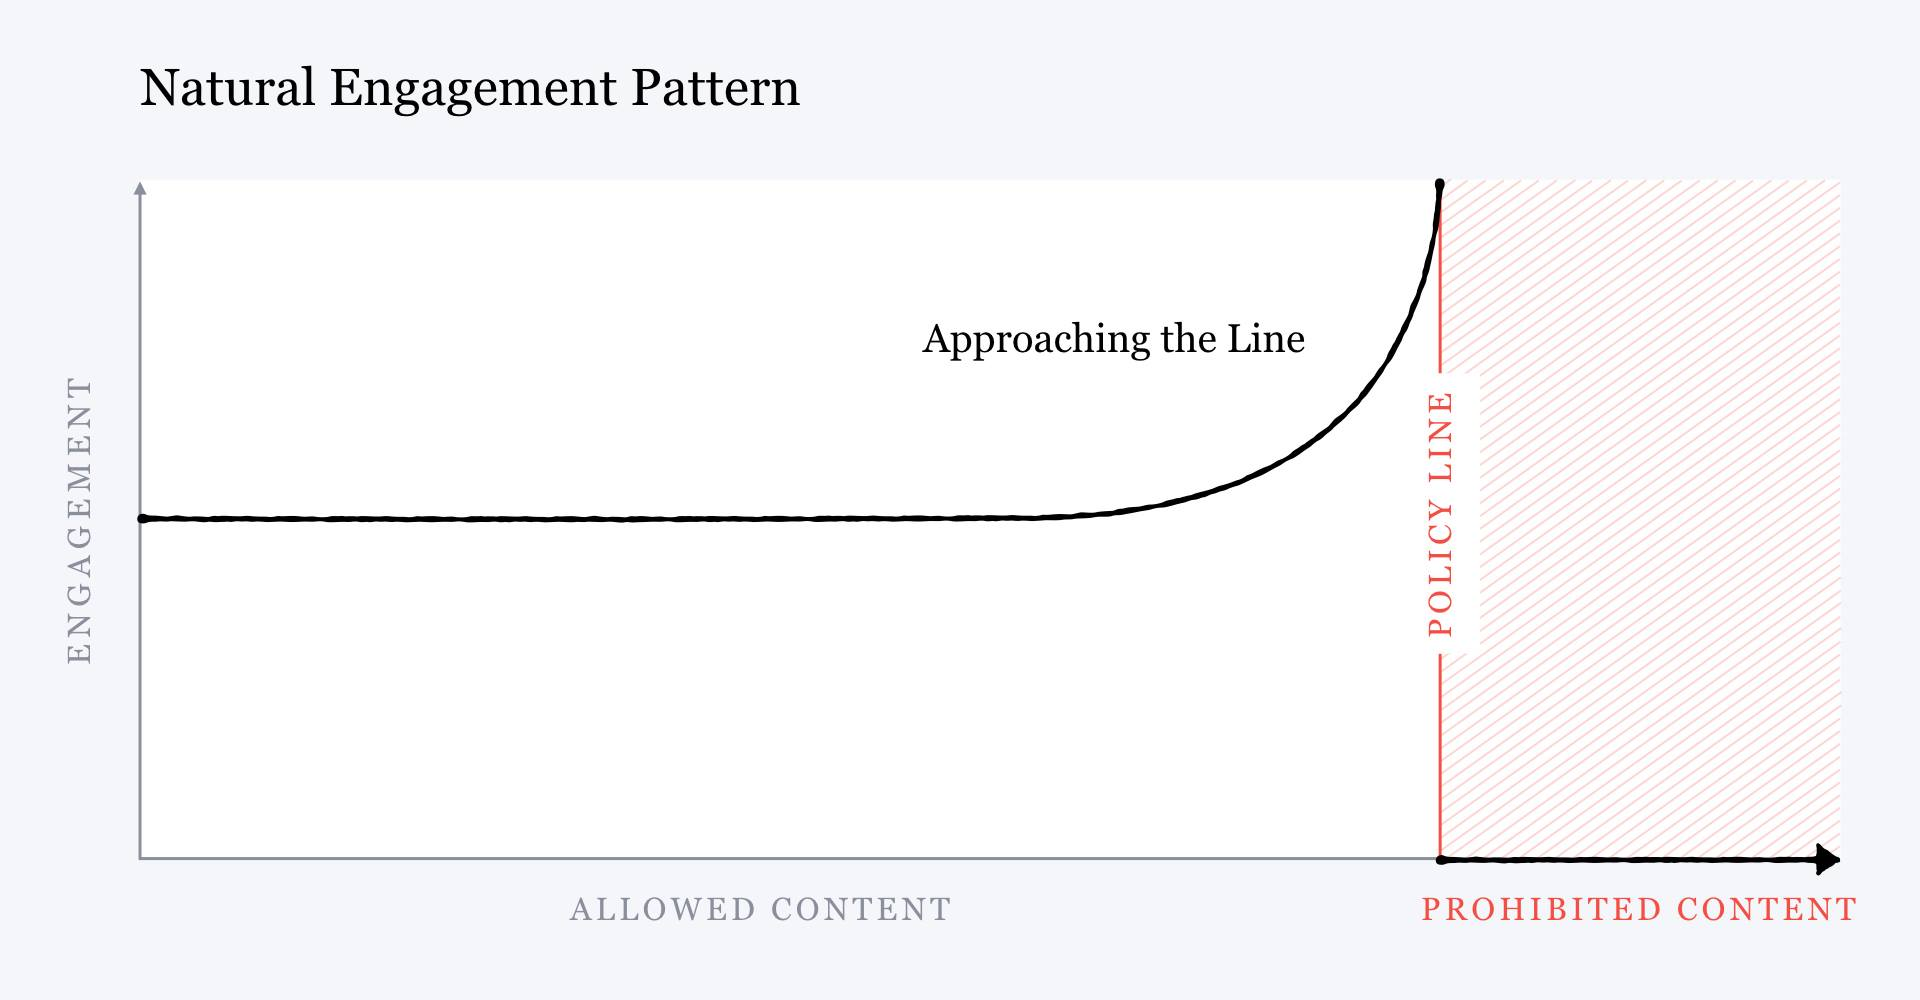
\includegraphics[width=\linewidth]{obrazky/fb_engagement.jpeg}
        \centering
        \label{fig:fb-enagement}
        \caption[Facebook Engagement]{Facebook Engagement. Zdroj: https://bit.ly/TRFBmisinformation}
    \end{figure}
    
    Aktuální studii, která se zaměřovala na volby v roce 2020, uskutečnili~\cite{edelson_nguyen_goldstein_goga_lauinger_mccoy_2021}, kteří došli k velmi podobným výsledkům jako výzkumné týmy Facebooku - politicky extrémní příspěvky mají tendeci generovat více uživatelských interakcí. Analýza se zaměřovala na interakci uživatelů s různými typy příspěvků, které vypadaly jako zpravodajství. 
    
    Monica Lee, výzkumnice a socioložka z Facebooku, v roce 2016 uvedla, že na Facebooku se nachází nejen velké množství extrémistických skupin, ale Facebook je navíc propaguje mezi svými uživateli. Až 64 \% uživatelů, kteří se přidali k těmto skupinám, tak učinili na základě doporučovacího systémů - výzvy typu „skupiny, které by se vám mohly líbit“ nebo „objevujte“. Během prezentace na mezinárodní bezpečnostní konferenci v Mnichově vedení společnosti prohlásilo, že se pokusí nedoporučovat skupiny, které jsou polarizující nebo porušují facebooková pravidla.~\citep{horwitz_seetharaman_2020} Problém doporučování extrémistických skupin tak podle všeho nebyl vyřešen ani v roce 2016, ani v roce 2018, kdy se jim zabývala pracovní skupina Chrise Coxe. 
    
    Zuckerberg i nadále přiznává, že Facebook může společnost rozdělovat a že je potřeba určitá míra regulace.~\citep{marson_2020} Na druhou stranu Facebook dosud prioritizoval svůj vlastní růst nad zájmy veřejnosti, a tak je řešení problémů zatím jen tak důležité, jak Facebook sám uzná za vhodné.~\citep{hao_2021}.

%%%%% ===============================================================================

\section{Doporučovací algoritmus - jak to funguje}
\label{chapter:doporucovaci-algoritmus-fungovani}
    Pochopit, jak doporučovací algoritmus Facebooku funguje je důležité nejen pro kontext výzkumu, který byl realizován v rámci této práce, ale také pro porozumění tomu, jaké máme možnosti v ohledu prevence a předcházení vzniku filtračních bublin.
    
    V první řadě stojí za facebookovým algoritmem sofistikovaný kód na bázi strojového učení~\citep{lada_wang_yan_2021}. Každá akce, která je na stránce uskutečněna, ať už komentář nebo like stránky, je využita k personalizaci uživatelské zkušenosti. ~\citep{satterfield_2020} 
    
    Příspěvky, které budou zobrazeny ve facebookovém „feedu“ určitého jedince jsou filtrovány několika stupňovým procesem za pomocí mnoha vrstev strojového učení. Cílem je zobrazovat takový obsah, který bude pro daného člověka relevantní, zajímavý a bude mu přinášet dlouhodobou hodnotu. To je určováno na základě řady faktorů jako: koho nebo co jsme nedávno začali sledovat, co jsme likovali nebo s čím jsme nedávno interagovali, co zajímá naše přátele\dots
    
    Facebooku především usiluje o to, aby uivatelům přinášel smysluplný obsah a vytvářel takzvané smysluplné interakce\footnote{V angličtině jako meaningful interactions.~\citep{facebook_2018} Jedná se o obecný koncept budování komunit, který se vyznačuje pozitivním vlivem na skupiny, ale i jednotlivce.~\citep{department2009guidance} }
    
    Obsahu, který je pro daného jedince relevantní mohou být stovky a tisíce, proto je nejdříve potřeba výběr zúžit a v konečném důsledku determinovat ty nejvýše postavené příspěvky. Na základě toho je vytvořeno několik samostatných modelů současně, které ohodnotí, co by se danému člověku mohlo nejvíce líbit - mohou být protichůdné a nesouhlasit spolu. Pro všechny je však ideálním cílem, aby daný jedinec provedl s doporučeným příspěvkem nějakou akci (engagement).
    
    Potom, co algoritmus každý příspěvek ohodnotí a přidá mu určité skóre, ověří integritu příspěvků - aby se mohly z výběru odfiltrovat fake news a „clickbait“ příspěvky - zúží výběr příspěvků na zhruba 500. Následně je znovu ohodnotí a seřadí podle skóre. Způsob tohoto hodnocení se pro každého může lišit - lidé s příspěvky různě interagují - někteří více likují, jiní zase sdílejí nebo komentují. Nakonec je provedena kontextuální kontrola, která zaručuje, že se ve „feedu“ zobrazí obsah různorodého charakteru (foto, videa, příspěvky, články\dots).~\citep{lada_wang_yan_2021}
    
    Ve zkratce by se celé hodnocení dalo rozvrhnout podle ~\citep{mosseri_2019}, do čtyř základních elementů: 
    \begin{enumerate}
      \item Dostupný \textbf{inventář} příběhů (příspěvků). 
      \item \textbf{Signály}, které jsou informačním základem pro hodnocení.
      \item \textbf{Předpověď} toho, jak se bude obsah líbit uživateli.
      \item \textbf{Skóre relevance} pro každý příběh.
    \end{enumerate} 
    
    Co se týče konkrétně fungování algoritmu, který vybírá stránky, které se zobrazí jako doporučené při zalikování jiné stránky, nelze s jistotou přesně říci, na jakých principech je postavený. Facebook na jednom ze svých webů jasně uvádí, že doporučuje stránky, skupiny a události na základě zájmů a akcí jednotlivých uživatelů tak, aby každý z nich dostával personalizovaná doporučení, která odpovídají jeho zájmům. Aby Facebook „ochránil“ uživatele od obsahu, který pro něj může být potenciálně nebezpečný nebo nevhodný, stanovuje si řadu pravidel pro doporučování obsahu.~\citep{rosen_2020}
    
    Za takový obsah může být považován obsah nízké kvality, nevhodný, obzvláště citlivý nebo nevhodný pro mladé publikum. Konkrétně existuje pět různých kategorií nežádoucího obsahu~\citep{facebook_2021B}:
    \begin{enumerate}
      \item Obsah, který brání podpoře bezpečné komunity (např. násilí, téma sebevraždy nebo poruch příjmu potravy, obsah sdílený nepodporovanou skupinou, obsah promující regulovaný produkt atd.).
      \item Citlivý obsah nebo obsah nízké kvality s tématem zdraví nebo financí (např. obsah, který zobrazuje kosmetické procedury; promování zavádějících business modelů atd. ). 
      \item Obsah, který uživatelů nemají rádi (např. „clickbait“ atd.).
      \item Obsah, který má nízkou kvalitu publikování (např. zprávy, které obsahují netransparentní informace o autorovi nebo vydavateli atd.)
      \item Nepravdivý nebo zavádějící obsah. (např. obsah, který byl shledán jako nepravdivý nezávislými lidmi/institucemi, které ověřují informace atd.) 
    \end{enumerate}
    
    \setlength\parskip{5mm}
    
    Facebook uvedl, že do ledna 2021 už deaktivoval tisíce skupin, které porušovaly jeho zásady komunity a šířily nepravdivý nebo nenávistný obsah. Proti stránkám, které (zatím) tvrdě neporušují pravidla Facebooku, ale jejich obsah může být potenciálně nebezpečný, se sociální síť rozhodla, mimo jiné, zasáhnout následujícími způsoby. Cílem je omezit formování těchto skupin na platformě~\citep{facebook_2021A}.
    \setlength\parskip{0mm}
    \begin{itemize}
        \item \textbf{Odstranění z Facebooku:} Neprodleně po tom, co se na stránkách objeví nepravdivý nebo nenávistný obsah.
        \item \textbf{Omezení doporučení:} Stránky nebudou doporučeny mezi podobnými stránkami. 
        \item \textbf{Zhoršit kvalitu vyhledávání:} Stránky nebude snadné na platformě dohledat.
        \item \textbf{Odstranění z Facebooku:} Neprodleně po tom, co se na stránkách objeví nepravdivý nebo nenávistný obsah.
    \end{itemize}

%%%%% ===============================================================================















%%%%% ===============================================================================

%%%\begin{table}[b!]

%%\centering
%%% The following packages are needed for this example:
%%%   - booktabs (\toprule, \midrule, \bottomrule)
%%%   - dcolumn (column type  D)
%%% Commands \pulrad and \mc defined in BcPrace.tex are used

%%%\begin{tabular}{l@{\hspace{1.5cm}}D{.}{.}{3.2}D{.}{.}{1.2}D{.}{.}{2.3}}
%%%\toprule
%%% & \mc{} & \mc{\textbf{Std.}} & \mc{} \\
%%% \pulrad{\textbf{Effect}} & \mc{\pulrad{\textbf{Estimate}}} & \mc{\textbf{error}$^a$} & 
%%% \mc{\pulrad{\textbf{P-value}}} \\
%%%\midrule
%%%Intercept     & -10.01 & 1.01 & \mc{---} \\
%%%Gender (male) & 9.89   & 5.98 & 0.098 \\
%%%Height (cm)    & 0.78   & 0.12 & <0.001 \\ 
%%%\bottomrule
%%%\multicolumn{4}{l}{\footnotesize \textit{Note:} 
%%%$^a$ Standard error of the estimator by the Monte Carlo method.}
%%%\end{tabular}%%%

%\caption{Maximum likelihood estimates from model M.}\label{tab03:Nejaka}

%%%\end{table}


%%%\textbf{Tables} should be formatted according to the following rules:
%%%\begin{compactitem} %% requires package paralist
%%%\item Avoid vertical lines. Separate the table from the surrounding
%%% text (even the legend) by stronger horizontal lines. Separate the
%%% header from the table and different parts of the table from each
 %%% other by thinner horizontal lines. This table format can be obtained
 %%% in \LaTeX\ by loading the package \texttt{booktabs}. If a stronger
 %%% separation of the columns is desired it can be achieved by including
 %%% an additional vertical space. 
%%%\item Do not change the type, format and meaning of the cells in a
%%%  single column (never include means in some cells and percentages in
%%%  other cells of the same column).
%%%\item Do not repeat the same cell contents many times. If the table
 %%% includes the column ``Variance'', which contains the value 0.5 in
  %%%the first ten cells and 1.5 in the next ten cells, delete this
 %%% column and find another way to communicate the value of the
 %%% variance. For example, the table can be divided into two separate
 %%% tables and the variance given in the legend. Or additional rows can
%%%  be included between the parts of the table informing what was the
%%%  variance in the subsequent rows.
%%%\item Numeric columns in the table should be aligned on the decimal
%%%  point. 
%%%\item Tables sometimes include abbreviations that are not used
%%%  elsewhere in the text. These abbreviations should be explained i%%% the legend or in notes under the table. These notes can be also used
 %%% to provide more detail on the meaning of selected columns or cells. 
%%%\end{compactitem}




%%%\section{Figures}

%%%Some advice on figures and diagrams:
%%%\begin{compactitem}
%%%\item Create the figure in the same size that will be used in the
%%%  thesis. Excessive magnification or reduction of figures causes poor
%%%  readability.
%%%\item The axes of a graph must be carefully annotated in the same
%%%  language the thesis is written in. Units of measurement (kg,
%%%  minutes, \ldots) should be provided when applicable. When the graph
%%%  plots a function $h(x)$ the axes should be annotated by $x$ a
%%%  $h(x)$. Each axis must have a clearly defined scale (tickmarks, labels).
%%%\item If a two-dimensional scatterplot includes a large number of
%%%  points make sure that the points do not turn into black cloud. If
%%%  the number of points is too large reduce the size of the plotting
%%%  symbol or select a subset of the points. Plots that include
%%%  thousands of points make problems in electronic documents, they
 %%% increase the size too much.
%%%\item If the thesis is to be printed on a black-and-white printer, do
%%%  not use colors. Lines can be distinguished by the type (solid,
 %%% dotted, \ldots), areas can be filled by various shades of grey or 

%%%The meaning of the line types and area shading should be explained in
%%%the legend or directly in the plot.
%%%\end{compactitem}





\chapter{Klimatická změna}
\label{chapter:klimaticka-zmena}
%\textcolor{green}{Kapitola nekompletní - 
    %Exituje nějaké skupina popíračů? Je to fenomén? Jak velký problém se z toho stal? je to vůbec problém? 
    %Filtrační bubliny a klimatická krize. Jaké jsou další studie? }

    Jak už bylo řečeno, kolem klimatické změny koluje spoustu dezinformací.~\citep{kolmes2011climate} Proto je nezbytné vymezit, co tento pojem znamená, co ho způsobuje a naopak s jakými pojmy bývá chybně zaměňován. Teoretické vymezení klimatické změny je také základem pro definici facebookových stránek, které se věnují klimatické krizi v následujících kapitolách. 
    
    Klimatická změna je definována dlouhodobou změnou v průměrných vzorcích počasí, které definují lokální, regionální a globální klima země. Pojem je často volně zaměňován s globálním oteplováním, nicméně hlavním rozdílem je, že klimatická změna označuje jak přirozené změny klimatu, tak ty, které jsou způsobeny člověkem.
    
    Klimatické změny, které byly vypozorovány od začátku 20. století, jsou převáž\-ně přisuzovány lidskému vlivu. Jedná se o spalování fosilních paliv, které způsobuje uvolňování skleníkových plynů do atmosféry a následně její rychlejší oteplování. Od před-idustriálního období se planeta oteplila o celý 1 °C, a toto číslo se v současnosti zvyšuje přibližně o 0.2 stupně každé desetiletí. 
    
    Je také důležité nezaměňovat klima s počasím. Počasí totiž označuje pouze atmosférické podmínky, které jsou lokální a krátkodobé povahy - vyznačují se sněhem, deštěm, mraky, větrem atd. Naproti tomu klima je dlouhodobého charakteru a pracuje s regionálními nebo celosvětovými hodnotami teploty, vlhkosti, srážkového úhrnu za dlouhé časové období - měsíce, roky, dekády.~\citep{nasa_2021}
    
    Jedním z důsledků klimatické změny je méně předvídatelné počasí, což může být obzvláště problematické pro státy, které jsou závislé na zemědělství a nekontrolovatelné změny počasí jim ovlivňují úrodu. Klimatické změny jsou také spojovány s dalšími živelnými událostmi jako jsou hurikány, záplavy, průtrže mračen nebo sněhové bouře. Na severu pak kvůli klimatickým změnám dohází k rychlejšímu tání ledovců, které způsobují stoupání hladiny moří v různých částech světa. 
    
    Jak už bylo zmíněno, klimatická změna je dvojí povahy - přirozená a způsobená lidmi. Ke změně klimatu tedy kontinuálně docházelo i dříve v historii. Jednalo se o pomalé a postupné změny, které trvaly stovky i tisíce let. Klimatické změny, které pozorujeme v současnosti, se však objevují v mnohem rychlejším tempu.~\citep{nationalgeographicsociety_2019}
    
    A právě kvůli rychlým změnám klimatu, které jsou (mimo jiné) charakterizovány nepředvídatelnými výkyvy počasí, zvyšováním hladiny oceánů nebo rizikem nedostatečných vodních zásob, mluvíme o klimatické krizi.~\citep{vitek_2020}
    
    Co je klimatická změna se nyní může zdát jako poměrně jasné, přesto existence antropocentrické (lidmi způsobené) klimatické změny vyvolává mezi veřejností živou debatu. Mimo jiné o tom, čím je charakterizována tato diskuze, co ji způsobuje a jak se vyznačují obě zainteresované strany pojednává následující kapitola.
    
%%%%% ===============================================================================
\section{Klimatická krize - filtrační bubliny a polarizace}
\label{sec:klimaticka-krize-bubliny}
    Přestože současná klimatická krize není novinkou a o její existenci se diskutuje již přibližně třicet let, za tuto dobu se nejen nepodařilo přijít na účinná řešení, která by klimatickou změnu zcela eliminovala (nebo alespoň výrazně zpomalila), ale dokonce se ani nepodařilo v tomto tématu dosáhnout konsensu u široké veřejnosti - jejíž jednotná kooperace je pro řešení problému důležitá. Ideologické odmítání klimatické krize se tak stalo předmětem řady studií napříč obory v posledních dvaceti letech.~\citep{almiron2019rethinking}
    
    Každý z nich nachází pro popírání klimatické krize své vlastní vysvětlení, ve kterém mají hlavní roli různí činitelé - od ziskuchtivého horního 1 \%, které ovlivňuje trh, až po jednotlivce, kteří nejsou schopni pochopit hloubku problému, a vyrovnat se s ním v kontrastu k jejich vlastním problémům každodenní reality.~\citep{mathers2020anthropology}
    
    Klimatická krize není izolovaným tématem, ale je zasazena do širšího kontextu toho, jaký názor má jedinec na jednotlivé politické otázky. To ovlivňuje způsob, jakým bude na celou problematiku nahlížet. 
    
    \setlength\parskip{5mm}
    
    \textit{„Studie ukazuje, že světonázor má malý, ale nezanedbatelný vliv na to, jakým způsobem je narativ klimatické krize zapamatován a převyprávěn. Výzkum mentál-ní reprezentace příběhu klimatické krize skrze třídění úkolů/klastrové analýzy odhalil, že ačkoliv obecná struktura zůstává stejná napříč světonázory, pouto mezi komponentem problému (krize kvůli klimatické změně) a navrhovaným řešením problému (strategie v boji s klimatickou změnou) se systematicky liší v závislosti na světonázor publika nebo mluvčího.“}\footnote{Přeloženo z: The present study shows that world views exert a small though non-negligible influence on how climate
    change narratives are remembered and retold. An examination of the mental representation of a climate change story via a
    sorting task/cluster analysis approach revealed that although the general story structure is very similar across world views, the
    link between the problem component (a crisis due to climate change) and the proposed problem solutions (strategies to
    counteract climate change) varies systematically as a function of the audience’s world view and of the speaker’s world view.}~\citep{bohm2019remembering}
    
    Klimatická krize proto může způsobovat vysokou míru polarizace. Lidé se dělí na „aktivisty“ nebo „skeptiky/popírače“. Diskuze na toto téma je charakterizována silnou homofilií založenou na daném postoji a rozdělením do stejně smýšlejících komunit, ze kterých uživatelé příliš nevystupují, aby se zapojili do opoziční diskuze. Lidé se silnými názory jsou také v diskuzích nejvíce slyšet.~\citep{WILLIAMS2015126} Proto je téma globální klimatické krize ideální živnou půdou pro vznik filtračních bublin a echo chambers.
    
    \setlength\parskip{0mm}
    
    Přestože „aktivisti“ i „skeptici/popírači“ mají jako svůj primární zdroj informací televizní zprávy, jejich sekundární zdroj se liší. Pro 17.8 \% „aktivistů“ jsou to televizní zprávy, pro 18.2 \% „skeptiků/popíračů“ jsou to exlusivně online dostupná média (jako např. Buzfeed, Huffington Post atd.). Klimatičtí skeptici také dávají větší přednost informacím z facebookové zdi nebo informacím, které sdílejí jejich přátelé a stránky tradičních novinových zdrojů (washingtonpost.com, nytimes.com atd.) jsou pro ně až na posledním místě. Dokonce jsou i za skupinou „další“ (blíže nespecifikované alternativní zdroje informací), které jsou sekundárním zdrojem až pro 10 \% z nich.  
    
    V otázkách klimatické změny pak můžou hrát právě zdroje pro čerpání informací důležitou roli.~\cite{carmichael} se ve své studii zabývají zvyšující se předpojatostí veřejnosti vůči problémům tohoto celospolečenského problému. Jejich zjištění potvrzuje hypotézu, že média mohou jedince utvrdit v jeho existujícím názoru, pokud přináší informace, které jsou s jeho vlastním pohledem konzistentní. Účastníci facebookové diskuze na téma klimatické krize mají tendenci soustředit se na jim blízký narativ a přehlížet jakýkoli jiný. Tím se vytváří struktura podobná echo chambers.
    
    Čím větší jsou rozdíly mezi sentimenty jednotlivých účastníků diskuze, tím větší je také polarizace~\citep{Zollo2019}. Stejné výsledky ukázala také studie realizovaná na sociální síti Twitter, která sledovala debatu okolo vydání IPPC\footnote{Integrated Pollution Prevention and Control v češtině Integrovaná prevence a omezování znečištění. Zpráva se zabývá právě klimatickou krizí.} zprávy z roku 2013. Tato studie potvrzuje, že se uživatelé častěji zapojují do debaty s lidmi, pokud sdílejí společný názor~\citep{pearce2014climate}.
    
    Podle dalšího průzkumu na vzorku americké veřejnosti se klimatičtí popírači vyznačují nižší mírou důvěry vůči vědecké komunitě oproti lidem, kteří v krizi věří.~\citep{krishna2021understanding} Neúměrné množství času a úsilí je tak v diskuzích na sociálních sítích věnováno nesouhlasu, pochybám nebo snaze dojít ke konsensu nad vědeckými otázkami klimatické krize, spíše než pokusu o nalezení přijatelných opatření proti tomuto problému~\citep{martin2014rebalancing}.
    
    Názory na klimatickou krizi, které jsou v rozporu s vědeckými výzkumy, se častěji objevují v zemích, kde odborníci na toto téma konsensu dosáhli. Hlasy klimatických skeptiků mohou být ve veřejné debatě přehlíženy, a proto tito lidé vyjadřují své názory v komentářích na internetu, kde se navzájem ve svých názorech utvrzují.~\citep{walter2018echo} 
    
    Facebook se v rocoe 2021 vyjádřil, že se pokusí bojovat proti dezinformacím, které jsou spojeny s klimatickou krizí a spustil na platformě ve Spojeném králov-ství testování nového systému, který by měl pomáhat vyvracet dezinformace. U některých příspěvků by měly být připnuty štítky, které budou uživatele odkazovat do repozitáře ověřených informací o klimatické změně. Podobný systém nedávno použili pro americké prezidentské volby 2020. Na tomto opatření by se měli podílet odborníci z celého světa. Společnost momentálně bojuje proti dezinformacím snižováním dosahu nepravdivých příspěvků.~\citep{hern_2021}
    
    Že je edukace v oblasti klimatické krize a snaha přesvědčit popírače o akutnosti tohoto tématu komplexním problémem, který nemá jednoduché řešení, dokazuje to, jak dlouho se už akademická obec tématikou zabývá bez většího výsledku. Například~\cite{nisbet2009communicating} už v roce 2009 navrhoval deduktivní soubor mentálních „zásuvek“ a interpretačních příběhů, který měl pomoci spojit publikum v otáz\-kách klimatické krize, a utvářet tak chování jednotlivců nebo mobilizovat kolektivní činy. Přesto i v roce 2021, o dvanáct let později, se ukazuje, že téma je stále aktuální. 
    
    Také proto se tato problematika stala námětem pro výzkum, který byl popsán v následujících kapitolách této práce. Ani v současné době, kdy máme v živé paměti rozsáhlé požáry v Australii a svět se potýká s globální pandemickou krizí, se nedaří veřejnost v otázkách klimatické krize sjednotit a dosáhnout konsensu~\citep{tarabay10,leyen_ghebreyesus_2020}. Následující kapitoly snad pomohou vyjasnit některé otazníky, které mohou viset nad fungováním filtračních bublin na facebookových stránkách, jež se zabývají klimatickou krizí.

%%%%% ===============================================================================



\chapter{Metodika}
\label{chapter:metodika}
    Součástí tohoto textu je obsahová analýza facebookových stránek, které se zabývají klimatickou krizí. Výzkumná část je postavena na třech výrocích či akcích Facebooku detailněji popsaných v kapitole~\ref{chapter:facebook} Sociální síť Facebook. Všechny tyto „výroky“ souvisí se vznikem filtračních bublin a jsou shrnuty do následujících bodů:
    \begin{enumerate}
        \item Facebooku usiluje o doporučování různorodého obsahu a tím předchází vzniku filtračních bublin. 
        \item Facebook se snaží omezovat šíření dezinformačních skupin.
        \item Stránky s větší mírou interakce se lépe šíří - vyšší míru interakce často mají stránky, které porušují zásady facebookové komunity. 
    \end{enumerate}
    
    Tato kapitola je krátkým úvodem do designu výzkumu, který vychází z těchto výroků. Kapitola stanovuje cíle a zasazuje výzkum do konkrét\-ního metodického rámce. 
 
 
\section{Cíl výzkumu}
\label{sec:cil-vyzkumu}
    Cílem výzkumu je zjistit, zda facebookový algoritmus napomáhá k prolamování informačních bublin na stránkách, které se zabývají klimatickou krizí.


\section{Výzkumná otázka}
\label{sec:vyzkumna-otazka}
    \setlength\parskip{5mm}
    
    První výzkumnou otázkou je: Pomáhá Facebook prolamovat filtračí bubliny doporučováním stránek s různým postojem ke klimatické krizi? 
    
    Druhou výzkumnou otázkou je: Jaká je frekvence doporučení stránek pro nebo proti klimatické krizi? 
    
    Třetí výzkumnou otázkou je: Jak se liší interakce na doporučovaných stránkách pro a proti klimatické krizi? 
    
    \setlength\parskip{0mm}


\section{Stanovení hypotéz}
\label{sec:stanoveni-hypotez}
    Jestliže se Facebook snaží předcházet vzniku filtračních bublin, mělo by se to projevit také v uskutečněném výzkumu. Abychom mohli dojít k jasným závěrům o filtarčních bublinách na Facebooku, byly stanoveny hypotézy, které vychází jak z cíle výzkumu, tak výzkumných otázek. 
    
    \setlength\parskip{5mm}
    
    H1: Facebook doporučuje všechny stránky o klimatické změně stejnou měrou bez ohledu na jejich postoj.
    
    \setlength\parskip{0mm}{}
    
    H2: Facebookový algoritmus posiluje vznik filtračních bublin na stránkách, které se věnují klimatické krizi.

\section{Motivace a význam}
\label{sec:motivace-vyznam}
    O filtračních bublinách se často hovoří v kontextu politické diskuze a rozhodování. Výskyt tohoto jevu však není omezen pouze na tuto konkrétní oblast, ale odráží se také na postojích ke klimatické krizi. 
    Ta se čím dál častěji stává tématem pro média, neboť se její dopady stále ve větší míře projevují v nejrůznějších koutech planety - příkladem mohou být rozsáhlé požáry v Austrálii na začátku roku 2020.~\cite{tarabay10}
    
    Rostoucí skepsi veřejnosti, která panuje vůči klimatické krizi, napomáhají filtrační bubliny, které utvrzují jedince v jeho vlastním postoji, a znemožňují mu tak získat různorodé podněty, které by mu umožnily informovanou změnu názoru.~\cite{carmichael} Společnost se tak rozděluje na dva tábory, které jen stěží docházejí ke konsensu.~\cite{WILLIAMS2015126} Ten je pro klimatickou krizi důležitý zejména proto, že skepse vůči tomuto tématu může mít negativní efekt na schvalování a důvěru vůči environmentálním opatřením, které se usilují o zmírnění negativních dopadů klimatické změny.~\citep{AKLIN2014173}
    
    \section{Výzkumná metoda}
    Použitou metodou bude obsahová analýza facebookových stránek s negativním a pozitivním postojem ke klimatické krizi. Obsahová analýza je jednou z nejdůležitějších výzkumných technik v humanitních vědách, která pohlíží na data jako na určitý druh komunikace s významem a kontextem, který je specifický pro dané publikum příjemců.~\cite{krippendorff2018content}
    
    \cite{Neuendorf} ve své knize uvádí, že obsahová analýza je numerickým procesem, jehož cílem je shrnutí dané skupiny zpráv. Nejedná se o abstraktní, ani detailní popis zprávy či skupiny zpráv. Jedná se tedy o kvantitativní analýzu. Přesněji o definuje obsahovou analýzu takto: 
    \setlength\parskip{5mm}
    
    \textit{
    „Obsahová analýza je shrnující, kvantitativní analýza zpráv, která se opírá o vědeckou metodu (včetně pozornosti vůči objektivitě-intersubjektivitě, předchozímu designu, reliability, validity, zobecnitelnosti, replikovatelnosti a testování hypotéz) a není omezena na typy proměnných, které lze měřit, nebo na kontext, ve kterém jsou zprávy vytvářeny či prezentovány.“}\footnote{Přeloženo z originálu: Content analysis is a summarizing, quantitative analysis of messagges that relies on the scientific method (including attention to objectivity-intersubjectivity, a prior design, reliability, validity, generalizability, replicability, and hypothesis testing) and is not limited as to the types of variables that may be measured or the context in which the messages are created or presented.} (s. 10)
    
    \setlength\parskip{0mm}


\chapter{Design výzkumu}
\label{chapter:design-vyzkumu}
    Facebook je prudce se rozvíjející platformou, která neustále mění, aktualizuje a zlepšuje algoritmy, které určují, co se bude na stránce dít a jaké bude mít funkce~\citep{hao_2021}. Přestože zástupci této společnosti přislíbili, že budou usilovat o větší transparentnost, je veřejnosti více méně skryto, jak přesně jednotlivé algoritmy fungují .~\citep{satterfield_2020}
    
    Na základě konkrétního předmětu výzkumu je tak méně či více snadné vyvinout metodiku pro danou studii. V průběhu sběru dat navíc může dojít k novým aktualizacím Facebooku, což může způsobit komplikace či úplnou ztrátu potřebných informací. Například v minulosti se design facebookových stránek několikrát změnil a s ním také možnosti přístupu k doporučovaným stránkám~\citep{facebook_2005, facebook_2020}. Například dříve bylo možné dohledat doporučené stránky ke konkrétní stránce za pomocí url adresy\footnote{https://www.facebook.com/pages/\linebreak?ref=page\_suggestions\_on\_liking\_refresh\&
    from pageid=}. Stačilo pouze za poslední rovnítko připsat ID požadované facebookové stránky. Následně se souhrnně zobrazily ostat\-ní, k ní doporučené, stránky. Takto už to dnes nefunguje a při vyzkoušení tohoto postupu je generován stále stejný seznam stránek bez jasné návaznosti na vstupní stránku.   
    Z toho důvodu byla pro cíle tohoto výzkumu vytvořena vlastní metoda postupu sběru dat a jejich vyhodnocení, která odpovídá současným podmínkám a výzvám Facebooku bez přímé replikace jiných studií.

%%------------------------------------------------------------------------
\section{Kategorizace dat}
\label{sec:kategorizace-dat}
    Před tím, než byl započat sběr dat a uskutečněna analýza facebookových doporučení, byly nejdříve definovány stránky, které jsou předmětem této analýzy. Přestože v cíli výzkumu jsou jednoznačně pojmenovány „stránky, které se zbývají klimatickou krizí“, tato definice je příliš obecná a do určité míry se mění v průběhu výzkumu, neboť na stránky se dá pohlížet z různých perspektiv.
    
    Na začátku proto byla potřeba rozdělit si stránky podle fáze, v které se ve výzkumu vyskytují: 
    
    \begin{enumerate}
      \item \textbf{Stránky vstupní (primární)}
    
        Jedná se pravděpodobně o tu nejdůležitější kategorii stránek, která byla vybírána záměrně a manuálně. Význam těchto stránek spočívá v tom, že jsou stavebním kamenem pro celou analýzu - vychází z nich všechna následují\-cí data.
        
        Vstupní stránky byly vybírány v angličtině, a to z toho důvodu, že tento výběr umožnil pracovat s větším množstvím stránek a tak přirozeně i větším množství dat. Práce s anglickými stránkami také otevírá možnost používat širší škálu nástrojů, které jsou často funkční pouze v angličtině. Jazyk byl v tomto ohledu jediným určujícím faktorem. Dále už nebyly stránky filtrovány podle konkrétní země - mezi primárními stránkami se proto nachází například mezinárodní stránka organizace Greenpeace, stránka vztahující se k obyvatelům Austrálie nebo stránka NASA z USA. Do výběru se mohla dostat i stránka jejíž správce se nachází v kterékoliv zemi na světě - jeho rodným jazykem nemusí být angličtina. Země původu tedy není určujícím kritériem.
        
        Aby se stránka dostala do primárního výběru, musí se nejen věnovat klimatické krizi, potažmo klimatické změně v antropocentrickém smyslu, ale důležitý je také postoj, který k tomuto tématu zaujímá. 
        
        Vstupní stránky, stejně jako sekundární a terciální, se dělí podle svého postoje ke klimatické krizi. Na jedné straně stojí \textbf{\uv{pro}} = s pozitivním postojem ke klimatické krizi - respektive takové, které souhlasí s existencí klimatické krize, která je způsobená lidmi. Na straně druhé jsou stránky s opačným postojem, tedy \textbf{\uv{proti}} = nesouhlasí s existencí klimatické krize, která je způsobená lidmi. Tyto stránky lze často (ne výlučně) považovat za dezinformační.
        
        Primární stránky byly vybírány tak, aby co nejpřesněji reprezentovaly dané postoje. Proto se jedná o stránky (především na straně \uv{proti}), které mají až extrémním vztah ke klimatické krizi - v případě \uv{proti} jsou to často stránky, které jsou až dezinformační a svůj postoj ke klimatické krizi velmi explicitně projevují - například se jej nesnaží sofistikovaně zaobalit do vědeckých dat. Dobrou ukázkou je stránka „Global Warming, Climate Change, whatever it's called is a scam“\footnote{Globální oteplování, klimatická změna nebo jak se to jmenuje je podvod.}, která svůj vztah k tématu klimatické změny vyjadřuje už ve svém názvu. 
        
        Stránky \uv{pro} jsou charakterizovány zejména tím, že se většinou jedná o stránky známých organizací (např. Greenpeace, NASA, Nature). Ale také jsou tyto stránky z větší části nositeli „modré fajfky“, která je oficiálním označením Facebooku pro pravost určité stránky. Ne ve smyslu pravosti informací, ale ve smyslu identity dané osoby či organizace. Stejné označení dostala i stránka CFACT, která se staví proti klimatické krizi.). I mezi vstupními stránkami \uv{pro} klimatickou krizi se nachází stránky vyjadřující svůj postoj. Například: Climate Change Is Real\footnote{Klimatická změna je opravdová.}. 
        
      \item \textbf{Stránky první úrovně (sekundární)} 
      
      Stránky první úrovně jsou takové stránky, které byly uvedeny jako doporučené na vstupních (primárních) stránkách. Mezi těmito stránkami se nacházely i takové, které jsou s klimatickou změnou zcela nesouvisející, proto byly v pozdější fázi výzkumu roztříděny, kategorizovány a případně vyřazeny.
      
      \item \textbf{Stránky druhé úrovně (terciární)} 
      
      Terciární stránky navazují na sekundární stránky. Jsou to tedy stránky, které byly uvedeny na předchozích stránkách první úrovně jako doporučené. Stejně tak byly roztříděny podle jejich souvislosti a vztahu ke klimatické krizi. Spolu se sekundárními stránkami jsou určujícím ukazatelem pro vznik nebo potlačení filtračních bublin. 
      \end{enumerate}
    
      Pokud u některých stránek první nebo druhé úrovně není na první pohled zcela zřetelné, zda patří do skupiny \uv{proti} nebo \uv{pro}, je vždy určující, zda klimatickou změnu v antropocentrickém pojetí přijímají nebo popírají. Například vyjadřování podpory nukleární energii nebo dokonce fosilním palivům ještě nutně neznamená, že je daná stránka proti - pouze to poukazuje na nekonvenční (oproti diskurzu klimatických aktivistů) přístup k řešení \citep{plumer_fountain_albeck-ripka_2018,carrington_2020}.
  
%%------------------------------------------------------------------------
\section{Nástroje analýzy a zdroje dat}
\label{sec:nastroje-analyzy}

Ke stažená dat a zpracování výsledků bude použito několik různých nástrojů. Tím uživatelsky nejjednodušším a nejběžnějším je Excel. Naopak tím uživatelsky nejnáročnějším je programovací jazyk Python\footnote{Stažení dat a částečné zpracování výsledků bylo umožněno spoluprací s programátorem.}. Dalším speciálním nástrojem je CrowdTangle, který posloužil ke stažení dodatečných dat z Facebooku.%i speciálními nástroji, které budou více popsány, jsou CrowdTangle a Voyant Tools. 

%\begin{enumerate}
   % \item Voyant tools
    
    %Voyant tools je volně dostupný software pro čtení a analýzu textů, který je možné používat skrze webovou aplikaci. Jeho kód je takzvaný „open-source“ (otevřený) a dostupný na serveru GitHub\footnote{https://github.com/sgsinclair/Voyant}. Je to původně akademický projekt, který je určený nejen pro akademiky, studenty digital humanities, ale i pro širokou veřejnost. 
    
    %Voyant Tools má téměř třicet různých použitelných nástrojů a umožňuje nejen počítačem asistovanou textovou analýzu, ale jeho funkce mohou být také přidány na různé webové stránky - blogy, časopisy a další. 
    
    %Aplikace pracuje hned s několika „open-source“ knihovnami a zakládá si na dostupnosti a jednoduchosti. Mezi designové principy patří také například modularit, flexibilita a mezinárodnost - Voyant Tools má mezi jinými také českou verzi.~\citep{voyanttools_2021}
    
    \subsection{CrowdTangle}
    
    CrowdTangle původně vznikl v roce 2011 nezávisle na Facebooku a svůj produkt vystavěl na veřejně dostupných API\footnote{Application Programming Interface - softwarový  prostředník, který umožňuje dvou aplikacím mezi sebou komunikovat. \citep{mulesoft_2021}}. Později v roce 2016 se společnost spojila s Facebookem a v současné době je služba považována za jednu z jeho aplikací.~\citep{matt_2016}
    
    CrowdTangle umožňuje jednoduše sledovat, analyzovat a následně pochopit, jak se obsah na sociálních sítích šíří a jaké jsou trendy nejen na Facebooku, ale také na Instagramu nebo Redditu. 
    
    Přesněji tento nástroj sleduje, kdy byl obsah zveřejněn, z jaké stránky či veřejného účtu byl zveřejněn nebo na jako stránku byl uveřejněn. Dále sleduje interakce, shlédnutí a sdílení. 
    
    Veřejně, bez registrace, je kromě rozšíření do prohlížeče, které umožňuje zjistit, kdo sdílel daný článek, dostupný také živý přehled, který umožňuje sledovat vývoj a konverzaci kolem specifických témat na Facebooku v reálném čase.
    
    Od roku 2019 CrowdTangle přizval do aplikace akademiky a vědce, aby jim umožnil lépe pochopit, jak se obsah na sociálních sítích šíří. Od toho si slibuje větší transparentnost Facebooku, která otevře online konverzaci a mimo jiné povede k větší bezpečnosti, spolehlivosti a přesnosti sociálních sítí. ~\citep{bleakley_2021}

%\end{enumerate}

%%------------------------------------------------------------------------
\section{Sledované položky}
  Ve chvíli, kdy byla shromážděna všechna potřebná data, bylo přistoupeno k samotné analýze. V první řadě je sledováno, jaké je zastoupení doporučovaných stránek a jakým způsobem jsou doporučovány. Konkrétně je sledováno:
  
\begin{itemize}
    \item Kolik je celkově zastoupeno stránek \uv{pro} a kolik \uv{proti}.
    \item Jak jsou stránky mezi sebou vzájemně propojeny. Neboli zda různorodým doporučováním dochází k prolamování informačních bublin.
    \item Které stránky jsou častěji doporučovány. Zda \uv{pro}, \uv{proti} nebo ekvivalentně. 
\end{itemize}
  
  Pro lepší porozumění sledovaných stránek a tomu, jak by mohl facebookový algoritmus stránky klasifikovat na základě jejich obsahu a interakcí, jsou sledovány především následující ukazatele: 
  
 \begin{itemize}
    \item Četnost interakcí na stránkách \uv{pro} a \uv{proti} 
    \item Druhy interakcí na stránkách \uv{pro} a \uv{proti}
    \item Druhy příspěvků na stránkách \uv{pro} a \uv{proti} (link, vlastní obsah atd.)
\end{itemize}
  

\chapter{Sběr a analýza dat}
\label{chapter:data}
    Celý výzkum je možné rozčlenit do pěti fází/kroků, z nichž některé jsou zautomatizované a jiné je nutné realizovat manuálně. Ke sběru a analýze dat byly použity nástroj CrowdTangle, která je více popsán v sekci~\ref{sec:nastroje-analyzy} Nástroje analýzy a zdroje dat.
    
    V této kapitole je rozepsán průběh celého výzkumu od výběru vstupních stránek, přes sběr potřebných dat až po závěrečnou analýzu dat. 

\section{Doporučení a výběr vstupních stránek}
\label{sec:vyber-vstup-stranek}
    Před začátkem analýzy byla důležitá snaha pochopit, jak doporučené stránky funguji a jak se zobrazují. Proto byl v počáteční fázi výzkumu proveden krátký pretest, který se zaměřoval na to, zda je vůbec možné sbírat data o doporučova\-ných stránkách, jakým způsobem a zda bude lepší pracovat s anglickými nebo českými stránkami. Tento pretest byl nezbytný i proto, že se v průběhu práce na tomto výzkumu změnilo prostředí Facebooku, a tedy i možnosti sběru dat. V úplných počátcích bylo ještě možné doporučené stránky filtrovat pomocí url adresy, jak je zmíněno v úvodu předchozí kapitoly~\ref{chapter:design-vyzkumu}, což se nakonec ukázalo jako nefunkční způsob. 
    
    Během pretestu se mimo jiné ukázalo, že aktualizace se odrazily také na způsobu, jakým se zobrazují doporučované stránky. To znamená, že doporučení již nejsou na stránce automaticky viditelná. Aby se zobrazil seznam doporučených stránek, je nejdříve potřeba dát like stránce, pro kterou chceme doporučení zobrazit, a až poté se rozbalí výběr doporučení ve vrchní části (viz Obrázek~\ref{fig:fb-likedoporucenestranky}). Tento seznam je zobrazen do té doby, než dojde k aktualizaci stránky nebo přesunu na jiné místo na Facebooku. Pokud chceme znovu zobrazit doporučené stránky, je potřeba na stránce like zrušit a následně ho znovu obnovit. Doporučené stránky jsou tedy zobrazovány pouze omezeně za dodržení určitých postupů.
    
    Stránky nejsou ukázány všechny najednou, ale ve skupinách po čtyřech (viz Obrázek~\ref{fig:fb-likedoporucenestranky}). Pro zobrazení dalších je vždy potřeba posunout se ve výběru šipkou doprava. Celkově je těchto doporučených stránek 19. Je sice možné kliknout na tlačítko, které slibuje zobrazení více doporučení, ale v tomto seznamu jsou všechny různé stránky bez ohledu na vztah k předešlé stránce. 
  
    \begin{figure}[H]
        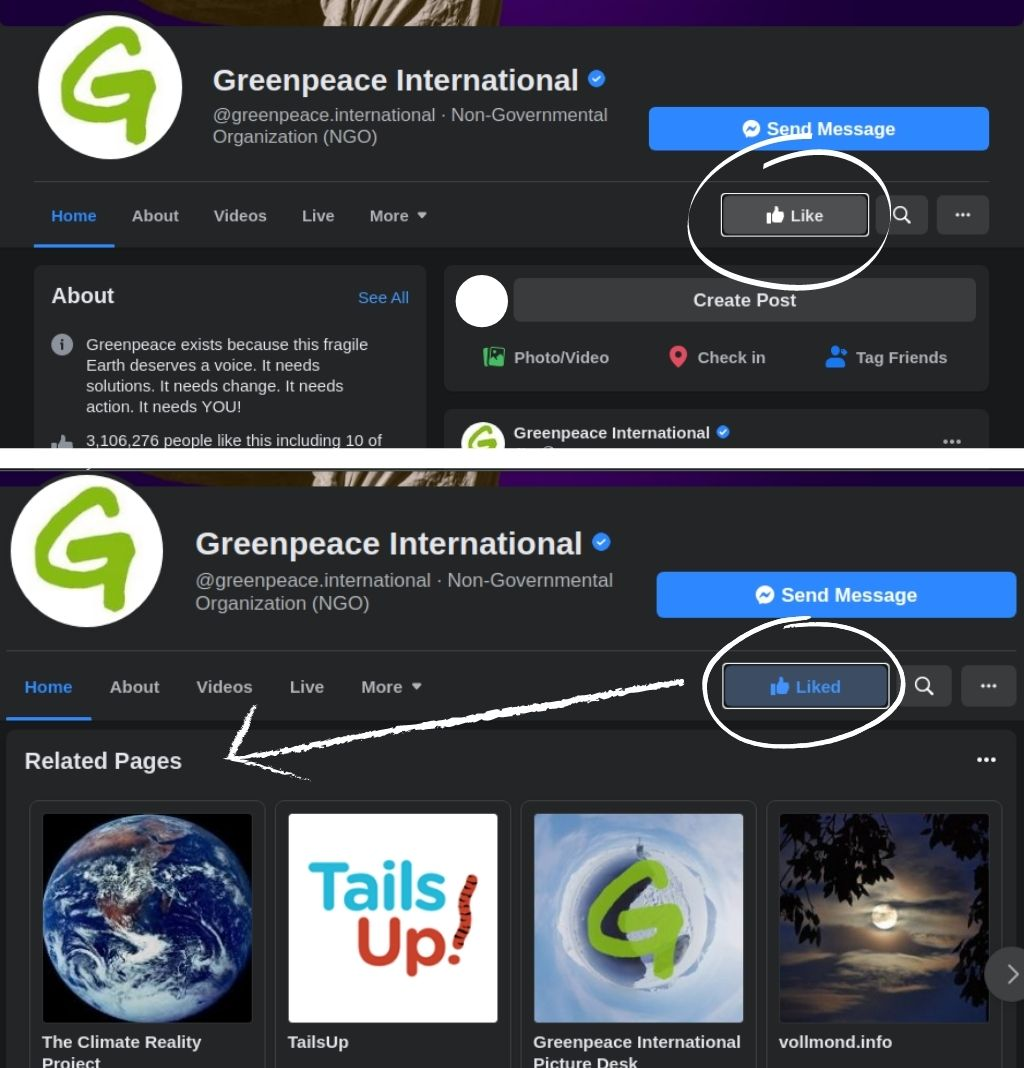
\includegraphics[width=\linewidth]{obrazky/like_doporucena (1).jpg}
        \centering
        \caption[Zobrazení doporučovaných stránek]{Zobrazení doporučovaných stránek. Zdroj: vlastní zpracování}
        \label{fig:fb-likedoporucenestranky}
    \end{figure}
  
    Není zcela jasné, podle jakého pravidla jsou stránky doporučovány. 19. března byl proveden test, kdy čtyři dobrovolníci propůjčili své profily a po zalikování totožných stránek se většině zobrazovaly prakticky totožné stránky jen s malými obměnami. O více než 20 dní později při testu na dalších třech osobách bylo v seznamu zobrazeno 11 odlišných stránek od těch z předchozího testu. Tito tři lidé však měli výčet doporučení na svých profilech také téměř totožný. Oba vzniklé seznamy doporučených stránek se prolínají. Nacházejí se v nich stránky, které mají podle tohoto pretestu silnou doporučovací hodnotu, neboť byly doporučeny všem zúčastněným, kteří poskytli náhled skrze své profily. Jsou to zejména ověřené stránky renomovaných organizací jako je Greenpeace, World Wild Fund, The Nature conservancy atd.  
    
    Výběr vstupních stránek probíhal manuálně dle kritérií stanovených v sekci \ref{sec:kategorizace-dat} Kategorizace dat. Předvýběr byl proveden už v rámci pretestu a následně byly vybrány pouze ty stránky, které nejvíce odpovídaly předurčeným požadavkům. Skrze funkci vyhledávání byla za pomoci klíčových slov cíleně provedena rešerše stránek \uv{pro} i \uv{proti} klimatické krizi. Vybrány byly první zobrazené výsledky odpovídající požadavkům - k tomu bylo potřeba stránku zobrazit a pečlivě prozkoumat její popis i obsah příspěvků. 
    
    Pokud tímto způsobem nebylo dohledáno odpovídající množství stránek, bylo použito právě rozšíření CrowdTangle pro prohlížeče, které umožňuje zjistit, jaké další stránky sdílely vybraný článek. Předpokladem je, že pokud například strán\-ka \uv{proti} sdílí protiklimatický článek, nabalí se další stránky s podobným postojem, které jej budou také sdílet. V krajním případě byly stránky vyhledávány skrze doporučení. Pokud již byla identifikovaná stránka \uv{proti}, skrze její doporučení byly vyhledány další podobné stránky. Vyhledávání stránek přes CrowdTangle a doporučení skrze již identifikované stránky bylo důležité především pro stránky \uv{proti}, které nebylo snadné dohledat přes facebookové vyhledávání.  
    
    Původně mělo být vybráno 10 stránek s pozitivním postojem a 10 stránek s negativním postojem ke klimatické krizi, ale během první fáze sběru dat se ukázalo, že jedna ze stránek \uv{proti} již zanikla a z toho důvodu již nebylo možné dále sbírat data. Proto byla náhodně odebrána jedna stránka z kategorie \uv{pro}. Z toho důvodu bylo nakonec vstupních stránek celkem 18. I při snížení počátečního vzorku stránek bylo stále možné získat dostatečné množství dat. 

    \setlength{\arrayrulewidth}{0.5mm}
    \setlength{\tabcolsep}{18pt}
    \renewcommand{\arraystretch}{2} 
     
    \begin{table}[h!] 
    \begin{center}
    \begin{tabular}{ | m{6cm}| m{5cm} | } 
    \hline
    \multicolumn{2}{|c|}{\Large \textbf{SEZNAM VSTUPNÍCH STRÁNEK}} \\
    \hline
    \textbf{stránky \uv{proti}} & \textbf{stránky \uv{pro}}  \\ 
    \hline
    CFACT & Greenpeace International \\ 
    \hline
    I Love Carbon Dioxide & NASA Climate Change \\ 
    \hline
    Climate Change LIES & Alliance for Climate Education \\ 
    \hline
    Australian Climate Madness & Climate Change Is Real \\ 
    \hline
    Climate Depot & Climate Reality \\ 
    \hline
    Climate Change Dispatch & Climate Change News \\ 
    \hline
    CO2 Coalition & Nature Climate Change \\ 
    \hline
    Global Warming, Climate Change, whatever it's called, is a scam. & Stop Global Warming \\ 
    \hline
    Global Climate Scam & Global Warming \\ 
    \hline
    \end{tabular}
    \caption{Seznam vstupních stránek}
    \label{table:seznam-vstupnich-stranek}
    \end{center}
    \end{table}
    
\section{Sběr stránek první a druhé úrovně}
\label{sec:sber-prvni-druha-uroven}
    Primární stránky jsou výchozím bodem pro další sběr dat. Jestliže každá (vstupní) stránka doporučuje až 19 dalších podobných stránek, to znamená při dvoustupňovém sběru dat tisíce stránek - přesněji až $19^2$. Zaznamenávat takové množství stránek manuálně by bylo přinejmenším časově náročné. Proto byla tato část (stejně jako některé další části) realizována strojově. 
    
    Strojový sběr dat byl uskutečněn za použití „scriptu“ v programovacím jazyce Python realizovaný s použitím knihovny Selenium, které umožňuje zautomatizování jednotlivých příkazů v interakci s prohlížečem.~\citep{pypi}. 
    
    Zjednodušeně proces vypadal asi takto: S pomocí knihovny Selenium se automaticky otevře prohlížeč a načte se jedna z vybraných vstupních Facebookových stránek. Aby bylo možné dát stránce like a zobrazit tak seznam doporučených stránek, je potřeba se přihlásit. Program se proto přihlásí k soukromému facebookovému účtu za pomocí osobních přístupových údajů (e-mail a heslo). Po zobrazení seznamu doporučených stránek je pro každou z nich stažen její název a url adresa. Nakonec je na každé stránce zrušeno likování. 
    
    Tento postup byl následně aplikován na každou další vstupní nebo sekundární stránku. Stahovány tedy byly doporučené stránky ze vstupních stránek - tzn. sekun\-dární stránky (18 stránek a na každé z nich 19 doporučených je 342) - a následně stránky doporučené na sekundárních stránkách - tedy terciární (342 stránek a na každé z nich 19 doporučených je 6 498 stránek). U těchto stránek druhé úrovně už dále nebyly zaznamenávány další doporučení. 
    
    Sběr všech dat nemohl proběhnout zároveň a najednou, ale musel být uskuteč\-něn ve třech fázích s jistými časovými rozestupy. Nedlouho po spuštění programu totiž narazil tento zautomatizovaný proces na bariéru Facebooku, která je vystavěna proti robotům a nevyžádaným strojovým akcím. Jinými slovy systém Facebooku rozpoznal, že aktivitu na stránkách neprovádí člověk, ale jiný algoritmus. Kromě varování ještě Facebook jako sankci za toto chování na několik dní zablokoval na účtu, který byl používán k přihlášení, možnost stránky likovat. Tato restrikce, ale byla za několik dní uvolněna a následně byl sběr dat preventivně rozložen do kratších úseků. 
    
    Aby mohly být všechny stránky později filtrovány a mohly být vybrány jen ty, které jsou pro výzkum relevantní, byl uskutečněn dodatečný sběr dat facebookových příspěvků. Pro všechny stránky v nově vytvořeném datasetu bylo za pomocí knihovny fb-scraper\footnote{https://github.com/kevinzg/facebook-scraper}, která umožňuje stahovat informace o veřejných stránkách bez API klíče, staženo přibližně třicet až čtyřicet příspěvků z jejich vlastního facebookového feedu, s cílem využít je v další fázi výzkumu~\citep{pypi_2021}. 
    
    \begin{figure}[H]
        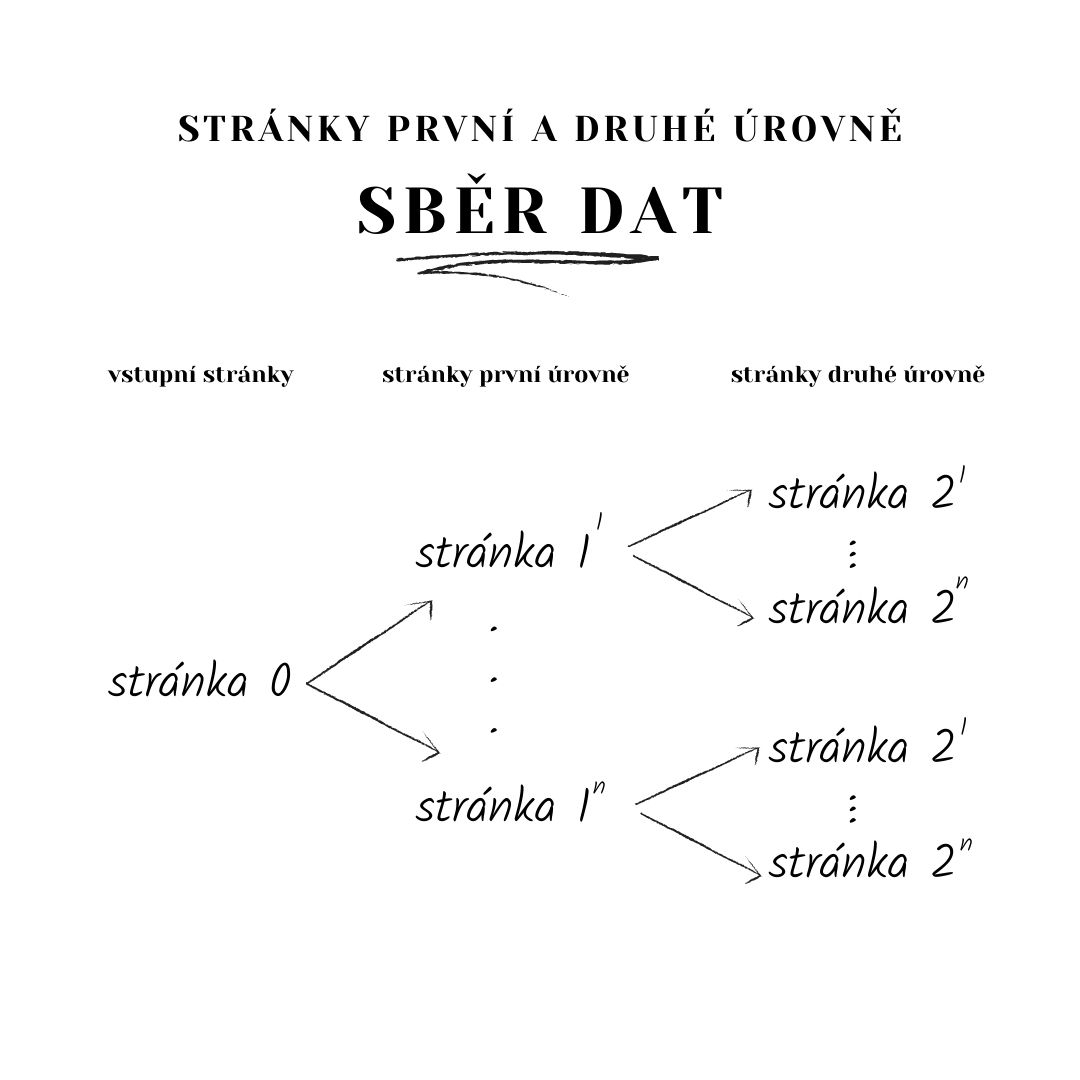
\includegraphics[width=\linewidth]{obrazky/sber_dat.jpg}
        \centering
        \caption[Schéma víceúrovňového sběru dat]{Schéma víceúrovňového sběru dat. Zdroj: vlastní zpracování}
        \label{fig:fb-sber-dat}
    \end{figure}
  
\section{Klasifikace stránek}
\label{sec:cisteni-klasifikace-dat}
    V doporučených stránkách se nemusí vždy nutně vyskytovat pouze stránky o klimatické krizi, ale mohou zde být i další podobné stránky (například takové, které spadají do stejné předdefinované kategorie facebookových stránek jako jsou třeba neziskové organizace nebo veřejně známá osobnost), proto byly vyfiltrovány a vyřazeny ty stránky, které se klimatickou krizí nezabývají. Tento krok je mimo jiné důležitý také pro následující fázi, ve které se stahuje mnohem větší množství příspěvků. Tímto včasným filtrováním se uspoří čas a prostor na pevném disku. Nakonec bylo nutné každou stránku klasifikovat jako \uv{pro} nebo \uv{proti} klimatické krizi. 
    
    Původně bylo zamýšleno, že ke kategorizaci dat v této fázi bude použit nástroj LIWIC\footnote{Zkrácený název pro Linguistic Inquiry and Word Count}, který slouží k analýze emocionálních, kognitivních a strukturálních komponentů nejen psaného textu. To se nakonec při bližším prozkoumání této metody ukázalo jako nevhodné a neúčinné.~\citep{pennebaker2015development} Místo toho byly použity jiné metody. Část tohoto procesu byla uskutečněna strojově a část manuálně se záměrem dosáhnout co nejpřesnějších výsledků. 
    
    Nejdříve bylo potřeba určit, které stránky nejvíce odpovídají tématu klimatické změny/klimatické krize. K tomu posloužily příspěvky, které byly staženy v předchozí fázi výzkumu. Tento balík přibližně třiceti až čtyřiceti příspěvků získaný pro každou ze stránek z datasetu (vstupní, sekundární, terciární) sloužil jako podklad pro klasifikaci. Klasifikace byla provedena na základě vytvořeného skóre, které určovalo, do jaké míry se stránka zabývá klimatickou krizí. 
    
    Před samotným výpočtem skóre a klasifikací bylo potřeba jazyková data (pří\-spěvky) předzpracovat. Za tímto účelem byly příspěvky tokenizovány - rozsekány na jednotlivá slova a převedena na malá písmena. Aby bylo dosaženo větší úspěš\-nosti při strojové identifikaci jednotlivých slov, byla všechny slova v příspěvcích lematizována. To znamená, že byla převedena na slovníkové tvary. Tato úprava umožňuje postihnout i případy kdy je slovo relevantní, ale není obsaženo v našich klíčových slovech. Pro ilustraci slovo going bude převedeno na tvar go. Následně byly odstraněny takzvané „stopwords“ - slova, které mají vysokou četnost a při zpracování přirozeného jazyka nepřinášejí téměř žádnou informaci, a proto se z textu odstraňují. Jinými slovy se jedná nadbytečná slova jako „the“, „a“, „it“ atd.  
    
    Pro předem definovaná klíčová slova \emph{climate, warming, CO2 a change} bylo vypočítáno vlastní skóre - pozitivní číslo, které vyjadřuje relevantnost daného příspěvku. Čím vyšší měla daná stránka toto skóre, tím více odpovídala tématu klimatické krize. 
    
    Je potřeba dodat, že výše zmíněná slova byla vybrána realizátorkou výzkumu na základě jejích osobních preferencí. Přestože byla vybrána taková slova, která podle ní nejvíce charakterizovala dané téma, tento výběr můžeme být zatížen určitým zkreslením. V nejhorším případě mohly být z výběru diskvalifikovány některé stránky \uv{pro} nebo \uv{proti}, které na svých stránkách častěji používají jiná slova, přestože mluví o klimatické krizi. 
    
    Skóre pro jednotlivé stránky byla počítána vlastním způsobem, který je kombinací klasického modelu TF-IDF\footnote{Term Frequency-Inverse Document Frequency je metoda, která měří, relevanci mezi texty a je typicky používaná pro vyhledávání v dokumentech.~\citep{ullman2011mining}} a BM25\footnote{BM25 je metoda, která také vrací relevanci mezi texty, ale provádí komplexnější výpočet.~\citep{article}}, respektive jeho TF částí. Nejdříve byly všechny příspěv\-ky pro danou stránku sloučeny do jediného dokumentu - tento postup byl následně proveden pro všechny stránky. V každém takovém dokumentu (specifickém pro každou ze stránek) byl vypočítán celkový počet výskytů klíčových slov (term-frequency). Aby výsledné skóre reflektovalo rozdílnou délku dokumentů (Krátký dokument obsahující stejný počet klíčových slov jako dlouhý dokument bude mít vyšší skóre.), byla tato četnost klíčových slov vynásobena vážícím koeficientem, který byl spočítán jako medián délky všech dokumentů a vydělen délkou dokumentu (počtem slov) specifického pro stránku, pro kterou bylo skóre počítáno. 
    
    Nakonec byl výsledný seznam stránek první a druhé úrovně (tedy bez osmnácti vstupních stránek) manuálně zkontrolován a každé ze stránek byla přiřazena „nálepka“ podle jejího vztahu ke klimatické krizi - to znamená \uv{proti} nebo \uv{pro}. Část stránek byla vyřazena pokud i přes tento postup neodpovídala definici stránek, které se zabývá klimatickou krizí. Některé stránky byly nakonec odstraněny neboť z nějakého důvodu již nebyly funkční či relevantní. Například stránku IISDRS není možné načíst a stránka REDD+ Ethiopia byla napadena hackery. 
  
\section{Stažení podrobných dat o příspěvcích}
\label{sec:stazeni-dodatecnych-dat}
    V neposlední řadě byla stažena dodatečná data ke všem stránkám, které se zabývají klimatickou krizí - stránkám, které prošly klasifikací a filtrováním v předchozím kroku. Tyto dodatečná data mohou posloužit k analýze souvislostí mezi doporučováním určité stránky a jejím obsahem nebo počtem interakcí. Například zda si vedou v oblasti interakcí lépe stránky \uv{pro} nebo \uv{proti} klimatické krizi.
    
    Ke stažení dodatečných informací o příspěvcích na všech stránkách, které vzešly z fáze očištění a klasifikace dat, byl použit nástroj CrowdTangle, který umožňuje analyzovat sociální sítě.~\citep{crowdtangle_2021} Dodatečná data obsahují informace o přibližně třiceti tisících příspěvků včetně názvu, ID a uživatel\-ského jména stránky nebo počtu „followerů“ v době zveřejnění příspěvku atd. Konkrétní informace o příspěvcích zahrnují mimo jiné datum zveřejnění příspěvku, počet a druh interakcí, druh příspěvku (video, foto, link\dots), url odkazu.   
  
\section{Analýza dat}
\label{sec:analyza-dat}
    Poslední, a zároveň tou nejdůležitější částí tohoto výzkumu je vyhodnocení dat s ohledem na výzkumné otázky a stanovené cíle. Analýza je založena na informacích, které byly získány na základě postupu, který byl popsán výše v této kapitole. 
    
    Včetně vstupních stránek zůstalo v datasetu po vyčištění celkově 280 unikát\-ních stránek. Z nichž pouhých 40 bylo proti klimatické změně a zbylých 240 mělo k této tématice kladný postoj\footnote{Způsob zařazení stránek viz kapitola 7.3 Očištění a klasifikace dat nebo více o kategorizaci dat v kapitole 6.1 Kategorizace dat.} Žádná z osmnácti vstupních stránek nebyla dále doporučena mezi stránkami první ani druhé úrovně až na Stop Global Warming, která se následně objevila přesně jednou (celkově tedy dvakrát). 
    
    V doporučení se (včetně duplikací) objevilo 658 relevantních stránek. Z toho 540 bylo s pozitivním vztahem k existenci klimatické změny a 147 s negativním postojem k existenci klimatické změny. 
    
    \begin{figure}[ht]
        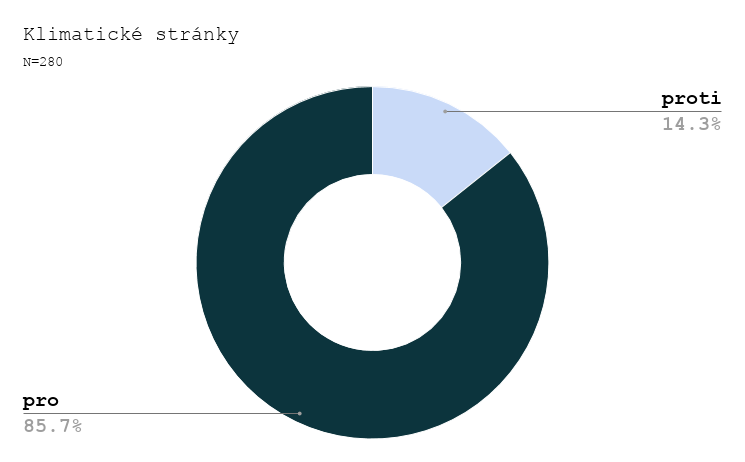
\includegraphics[width=11cm]{obrazky/Klimatické stránky N=280.png}
        \centering
        \caption[Poměr klimatických stránek podle kategorie]{Poměr klimatických stránek podle kategorie. Zdroj: vlastní zpracování}
        \label{fig:fb-klima-stranky-kategorie}
    \end{figure}

    Přestože je stránek \uv{proti} šestkrát méně než stránek \uv{pro}, v celkovém datasetu doporučených stránek se častěji opakují oproti stránkám \uv{pro}. Což může být právě tím, že těchto stránek není tolik, a proto má Facebook menší výběr stránek, ze kterých může pro doporučování čerpat. Zatímco stránky \uv{pro} se objevují v doporučení průměrně přibližně dvakrát, stránky \uv{proti} více než třikrát. Zatímco v první úrovni je doporučeno 21 unikátních stránek \uv{proti} v další úrovni už je to jen 10 unikátních stránek. Doporučení negativních stránek je tedy prakticky vyčerpáno už mezi vstupními daty a daty první úrovně.  

    \begin{figure}[H] 
        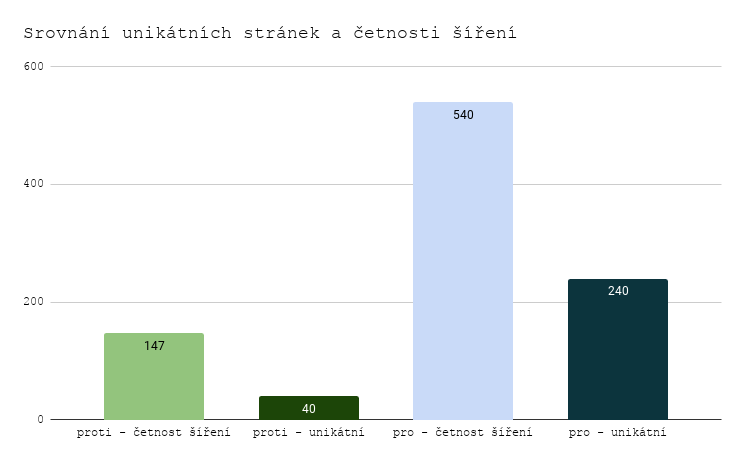
\includegraphics[width=14cm]{obrazky/Srovnání unikátních stránek a četnosti šíření.png}
        \centering
        \caption[Srovnání unikátních stránek vzhledem k četnosti šíření]{Srovnání unikátních stránek vzhledem k četnosti šíření. Zdroj: vlastní zpracování}
        \label{fig:fb-klima-stranky-sireni}
    \end{figure}

    Konkrétně je v celém datasetu stránka s pozitivním postojem k existenci klimatické změny průměrně doporučována 2,25x s medianem 1 a stránka s negativním postojem ke klimatické změně 3,68x se střední hodnotou 3. S tím, že nejčastěji je u obou kategorií stránka doporučena pouze jednou. 
    
    Méně než polovina všech stránek (bez ohledu na postoj ke klimatické změně), přesněji 134, byla doporučena více než jednou. Pouze 25 stránek mělo více než 5 doporučení a jen 8 stránek mělo 10 a více. Konkrétní seznam stránek těchto osmi stránek je možné si prohlédnou v tabulce~\ref{table:nejcasteji-sirene-stranky} Nejčastěji šířené stránky. 
    
    Jedná se o stránky jak velkých mezinárodních organizací jako je Greenpeace nebo Organizace spojených národů, tak o menší stránky se středním i nižším počtem followerů. Na první pohled vyčnívá stránka Lord~Monckton, která má vzhledem k ostatním stránkám jen okolo 9,5 tisíc sledujících a zároveň ve svém názvu nijak nenaznačuje spojitost s klimatickou změnou - ovšem při bližším prozkoumání stránky a jejích příspěvků je vidět, že toto téma je často zmiňováno jak v příspěvcích, tak v samotném popisu stránky, kde je Lord~Monckton označován jako odborník na klimatickou změnu. Jako svou webovou stránku taktéž uvádí web CFACT, který může být považován za proti klimatický portál. Další stránkou, která se výrazně vyčnívá je Above~Climate~Change s pouhými 367 followery. 
    
    Přestože jsou stránky s negativním postojem ke klimatické změně doporučová\-ny více (z pohledu frekvence doporučování) než stránky pro klimatickou změnu, mezi výběr osmi nejšířenějších stránek se dostalo více \uv{pro} nežli \uv{proti}. Konkrétně je rozložení stránek v poměru 5:3. Vysvětlení může být více: ať už celkově výší počet followerů u stránek \uv{pro} nebo lepší publicita a větší kredibilita stránek velkých organizací jako je Greenpeace nebo OSN.

    \setlength{\arrayrulewidth}{0.5mm}
    \setlength{\tabcolsep}{25pt}
    \renewcommand{\arraystretch}{2} 
    
    \begin{table} [h!] 
    \centering
    \resizebox{\textwidth}{!}{
    \begin{tabular}{| m{4cm}| m{1.7cm} | m{1.2cm} | m{1.7cm} |} 
    \hline
    \multicolumn{4}{|c|}{\Large \textbf{8 NEJŠÍŘENĚJŠÍCH STRÁNEK}}   \\ 
    \hline
     \textbf{Název stránky} & \textbf{Vztah ke klimatické krizi} & \multicolumn{1}{c|}{\textbf{Doporučení}} & \multicolumn{1}{c|}{\textbf{Followers}}            \\ 
    \hline
    Lord Christopher Monckton, 3rd Viscount Monckton of Brenchley & proti & 17 & 9 444 \\ 
    \hline
    Friends of Science & proti & 14 & 34 198 \\ 
    \hline
    Skeptical Science & pro & 13 & 183 498 \\ 
    \hline
    Inside Climate News & pro & 13 & 81 086 \\ 
    \hline
    Climate Home News & pro & 12 & 18 810 \\ 
    \hline
    Above~Climate~Change & proti & 10 & 367 \\ 
    \hline
    Greenpeace USA & pro & 10 & 726 174 \\ 
    \hline
    UN Environment Programme & pro & 10 & 1~094~527 \\
    \hline
    \end{tabular}
    }
    \caption{Nejčastěji šířené stránky}
    \label{table:nejcasteji-sirene-stranky}
    \end{table}

\subsection{Prolomení bubliny}
\label{sec:prolomeni-bubliny}
    K pochopení, jakým způsobem je analyzováno prolomení filtrační bubliny, je důležité porozumět tomu, že prolomení může být identifikováno pouze existuje-li spojení mezi výchozí stránkou a dalšími stránkami, které doporučuje. Těmito výchozími stránkami mohou být v tomto případě pouze stránky vstupní a první úrovně. Těchto stránek, nepočítáme-li jejich duplikace, je v kategorii \uv{pro} 67 a v \uv{proti} 20. Zbylé stránky jsou stránky druhé úrovně u kterých už nejsou v rámci tohoto výzkumu uvažovány/promítnuty žádné další doporučení. Proto mají stránky druhé úrovně spíše referenční funkci ke stránkám první úrovně. 
    
    Při prozkoumání „větve“ doporučení, která vychází ze vstupních stránek akceptujících existenci klimatické krize, se ukazuje, že jsou zde doporučovány téměř výhradně stránky se stejným postojem. V celém řetězci (mezi první a druhou úrovní) se objevuje jen 7 stránek \uv{proti} klimatické změně a na druhou stranu je zde doporučeno 429 stránek se stejným postojem jako mají vstupní stránky. Na každou stránku bylo průměrně doporučeno přibližně 6.5 relevantních stránek. Z toho průměrně 6.3 bylo \uv{pro} a jen 0.1 \uv{proti}, což vypovídá o téměř nulovém prolomení filtrační bubliny. 
    
    Stránky, které souhlasí s existencí klimatické změny a byla u nich prolomena filtrační bublina, jsou v porovnání k některým ostatním stránkám \uv{pro} vzhledem k počtu fanoušků spíše střední, až menší velikosti. Nejedná se o stránky se statisící fanoušky a jsou zde stránky, které mají jen několik tisíc followerů. Stránka s největším počtem fanoušků má 60 600 a stránka s nejmenším počtem jen 2 280.
    
     \setlength{\arrayrulewidth}{0.1mm}
    \setlength{\tabcolsep}{40pt}
    \renewcommand{\arraystretch}{1}
    \begin{table}[h!] 
        \centering
        % \resizebox{\textwidth}{!}{%
        \begin{tabular}{| m{2cm} | m{1.7cm} | m{2cm} |} 
            \hline
            \multicolumn{3}{|c|}{\Large \textbf{Prolomení bublin stránky \uv{pro} }} \\ 
            \hline
            \textbf{Název stránky} & \textbf{Počet prolomení} & \textbf{Followers} \\ 
            \hline
            Citizens Climate Lobby  & 1 & 41 471 \\ 
            \hline
            I Heart Climate Scientists  & 1 & 60 601 \\ 
            \hline
            Global Warming Fact of the Day  & 1 & 10 927 \\ 
            \hline
            Our Children's Trust  & 1 & 29 640 \\ 
            \hline
            Global Warming Climate Change Report  & 1 & 13 524 \\ 
            \hline
            Climate Change is Real  & 1 & 2 280 \\ 
            \hline 
            Mothers for Nuclear  & 1 & 6 590 \\ 
            \hline
        \end{tabular}%
        % }
        \caption{Stránky \uv{pro}, v jejichž doporučení byla prolomena bublina.}
        \label{table:prolomeni-bubliny-pro}
    \end{table}
    
    Stránky \uv{proti}, které prolomily filtrační bublinu stránek s pozitivním postojem k existenci klimatické změny byly pouze čtyři - Climate Change Facts, Refutations to Anti-Nuclear Memes, The Global Warming Policy Forum, Dr. James E. Hansen. - z nichž 3 prolomily každá jednu stránku \uv{pro} a jedna ze stránek opakovaně prolomila více stránek. Jednalo se o stránku Dr. James E. Hansen. 
    
    Při sledování vývoje doporučení vycházejícího ze vstupních stránek, které popírají existenci klimatické krize, jsou výsledky příznivější ve prospěch prolamování filtračních bublin. Relevantních stránek je v tomto případě méně, průměr\-ně 4.8, a připadá na ně zhruba 3.4 proti klimatických stránek. Což je sice pořád hodně, ale na druhou stranu každá stránka (vstupní nebo první úrovně) doporučuje v průměru 1.5 stránky s opačným postojem ke klimatické krizi. Takže z každého doporučení je teoreticky možné dostat se alespoň na jednu stránku s opačným názorem na toto téma. V praxi ale některé stránky \uv{proti} doporučují více stránek \uv{pro} a z toho důvodu jen u patnácti stránek \uv{proti} dojde k prolomení filtrační bubliny.
    
    Stránky, které nesouhlasí s existencí klimatické změny mají obecně méně fanoušků než stránky s opačným postojem. Vzhledem k tomu, že nad otázkami klimatické změny panuje vědecký konsensus, je logické, že odpůrců tohoto postoje je menšina. Narozdíl od stránek \uv{proti} se mezi stránkami \uv{pro}, jak už bylo řečeno, nachází i stránky velkých známých mezinárodních organizací, které mají statisíce fallowerů. V kontrastu jedna z největších stránek, která jde proti klimatu s názvem CFACT, má jen 61 157 followerů. Proto i v tabulce prolomení filtračních bublin stránek \uv{proti} jsou spíše stránky menší velikosti. Rozpětí je však velmi široké od 464 fanoušků až po 34 188. Dvě nejmenší stránky také dostaly dvě nejvyšší prolomení. 
    
    \setlength{\arrayrulewidth}{0.5mm}
    \setlength{\tabcolsep}{60pt}
    \renewcommand{\arraystretch}{1.5} 
    
    \begin{table} [ht] 
    \centering
    \resizebox{\textwidth}{!}{%
    \begin{tabular}{| m{4cm}| m{1.5cm} | m{2cm} |} 
    \hline
    \multicolumn{3}{|c|}{\Large \textbf{Prolomení bublin stránky \uv{proti} }}   \\ 
    \hline
    \textbf{Název stránky} & \textbf{Počet prolomení} & \textbf{Followers}            \\ 
    \hline
    Climate Change Facts  & 10 & 464 \\ 
    \hline
    The Global Warming Policy Forum & 5 & 14 124 \\ 
    \hline
    Climate Change and Global Warming - Exposed  & 5 & 528  \\ 
    \hline
    Is There Global Cooling  & 4 & 2 525 \\ 
    \hline
    Climate Change Dispatch  & 3 & 6 036  \\ 
    \hline
    Climate Change LIES  & 3 & 16 238  \\ 
    \hline
    Climate News  & 3 & 3 149 \\ 
    \hline
    I love Carbon Dioxide  & 2 & 19 847 \\ 
    \hline
    wattsupwiththat  & 2 & 13 017 \\ 
    \hline
    Global Climate Scam  & 2 & 1 254 \\ 
    \hline
    CO2 Coalition  & 1 & 6,056 \\ 
    \hline
    World Wide Protest Against the Global Warming SCAM  & 1 & 1 152 \\ 
    \hline
    Center for Industrial Progress  & 1 & 5 749 \\ 
    \hline
    Global Warming, Climate Change, whatever it's called, is a scam.  & 1 & 1 611 \\ 
    \hline
    Friends of Science  & 1 & 34 188 \\ 
    \hline
    \end{tabular}%
    }
    \caption{Stránky \uv{proti}, v jejichž doporučení byla prolomena bublina.}
    \label{table:prolomeni-bubliny-proti}
    \end{table}
    
    Mimo jiné je zajímavé, že se počty prolomení u stránek jeví bez na první pohled jasného vzorce. Stránka Climate Change Facts má 10 opačných doporučení, zatímco stránky Climate Change and Global Warming - Exposed a The Global Warming Policy Forum, které jsou v počtu prolomení na druhém místě, mají jen 5 názorově odlišných doporučení. Následně už doporučení klesají vždy o jedno číslo. Vysvětlení tohoto jevu by mohlo být v zásadě jednoduché. Některé stránky se v datasetu opakují, a tudíž mají teoreticky i větší šanci několikrát prolomit filtrační bublinu.
    
    Doporučení by se také mohly odvíjet od názvů stránek. Například stránka Climate Change Facts na první pohled vypadá jako stránka, které pravdivě informuje o klimatické změně. To by mohlo být jedno z vysvětlení pro skokový rozdíl v doporučení oproti ostatním stránkám.
    
    Jedná se však o pouhou domněnku, která pravděpodobně nebude jediným faktorem, který hraje v doporučení roli. Mezi stránkami, které bublinu prolomily, jsou totiž i takové, které už ve svém názvu vyjadřují jasný nesouhlasný postoj ke klimatické změně. Jsou to stránky Climate Change LIES; Global Climate Scam; World Wide Protest Against the Global Warming SCAM; Global Warming, Climate Change, whatever it's called, is a scam. Několik stránek pak svůj postoj vyjadřuje nepřímo, například zaobalením do ironie jako: Is There Global Cooling nebo I love Carbon Dioxide. Název by mohl být pro zařazení stránek významný - vyjádření postoje by mohlo třídění doporučení usnadnit a při použití ironie nebo věrohodného názvu by naopak mohla být stránka zařazena chybně. 

    
    Stránek, které prolomily filtrační bublinu na stránkách, které se vyhraňují proti existenci antropocentrické klimatické změny, bylo celkově třicet dva. Osmi z nich se podařilo bublinu prolomit u více než jedné stránky. Z nich u dvou byly prolomeny tří a u jedné čtyři stránky. Nejúspěšnější stránky v tomto prolamování byly v pořadí od nejvíce prolomení po nejméně tyto stránky: Skeptical Science, Climate Home News, Bulletin of the Atomic Scientists, Mothers for Nuclear, Climate Change In Pictures, Global Warming Planet, Global Warming Times, Climate Discussion Nexus.
    
    \begin{figure}[H]
        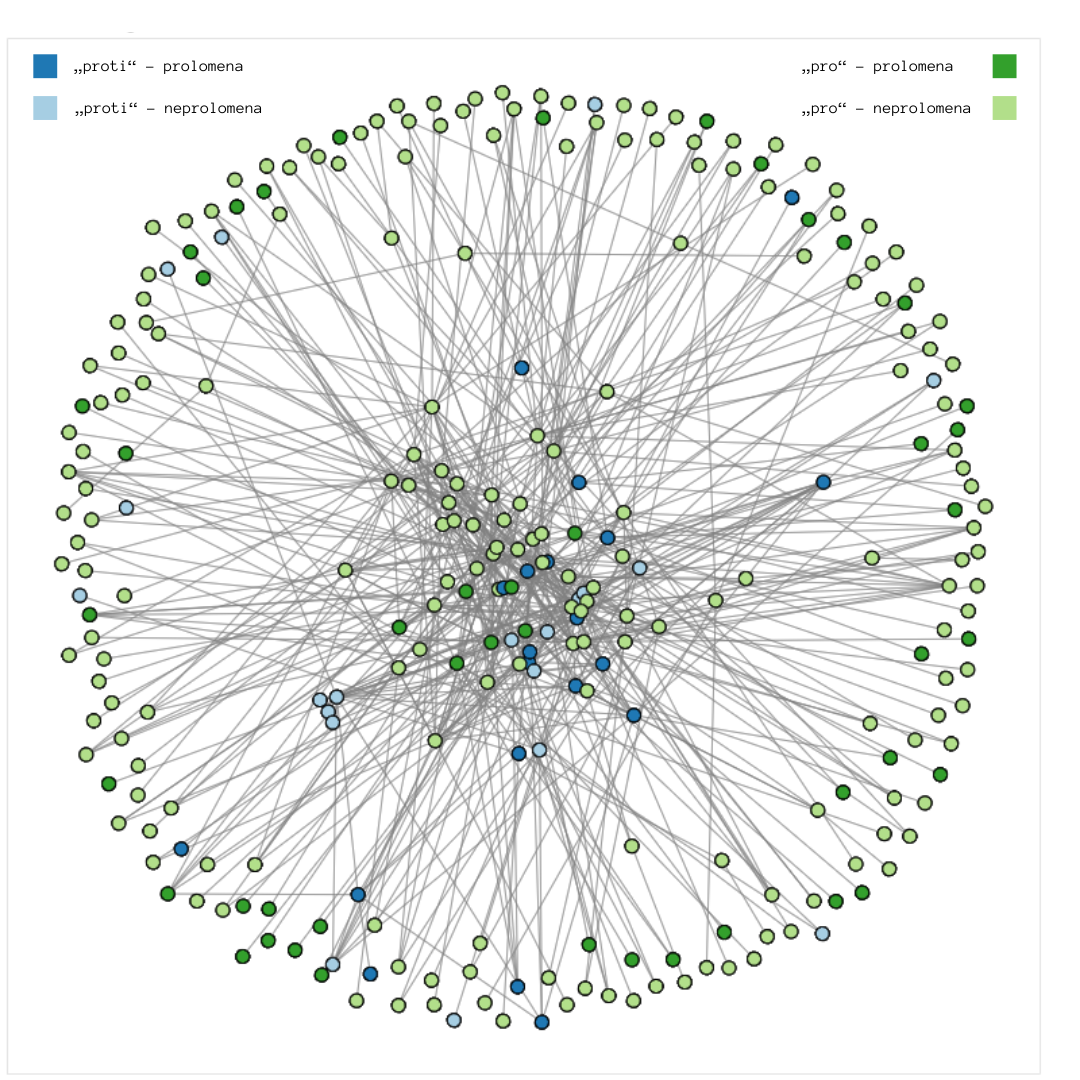
\includegraphics[width=13cm]{obrazky/prolomenibublinymapa_spopisky.png}
        \centering
        \caption[Mapa prolomení filtračních bublin]{Mapa prolomení filtračních bublin. Zdroj: Vlastní zpracování}
        \label{fig:fb-klima-stranky-bubliny}
    \end{figure}
    


%-------------------------------------------------------------------------------

\subsection{Interakce na stránkách a jejich příspěvky}
\label{sec:interakce}
    Pro lepší porozumění tomu, zda může mít na četnost šíření stránek a prolamování filtračních bublin vliv engagement, jak bylo naznačeno v sekci~\ref{sec:doporucovaci-algoritmus-engagement} Doporučovací algoritmus - za vším hledej engagement, byla také provedena analýza, která se zaměřovala na reakce na stránkách s pozitivním i negativním postojem ke klimatické změně. 
    
    Jak se ukazuje, stránky \uv{pro} mají v průměru asi jednou tolik interakcí na stránku, jako stránky \uv{proti}. Konkrétně je to 14 746 ku 6 968. U stránek \uv{pro} je průměrně 105 interakcí a u stránek s negativním postojem k existenci klimatické změny je to 67 na příspěvek. 
    
    V potaz však musí být brán i počet followerů na stránkách s pozitivním i negativním postojem k existenci klimatické krize. Stránky \uv{pro} mají v průměru téměř $36\times$ více fanoušků než stránky \uv{proti}. A zatímco na každého fanouška stránky \uv{pro} připadá průměrně 0.0012 reakcí, na každého fanouška stránky \uv{proti} je to 0.0065 reakcí. Lidé, kteří sledují stránky s negativním postojem k existenci klimatické změny, tedy s příspěvky interagují více. 
    
    %Při bližším pohledu na průměr jednotlivých reakcí\footnote{Angry, sad, shares, love, wow, care, comments, haha a likes.} stránky \uv{pro} nedosahují v žádném z případů ani poloviny průměrných hodnot stránek s pozitivní postojem k existenci klimatické změny. Nejvíce se stránky \uv{proti} blíží stránkám \uv{pro} v průměrných hodnotách interakcí v použití reakcí „haha“, sdílení a komentář. 
    
    %\begin{figure}[H]
        %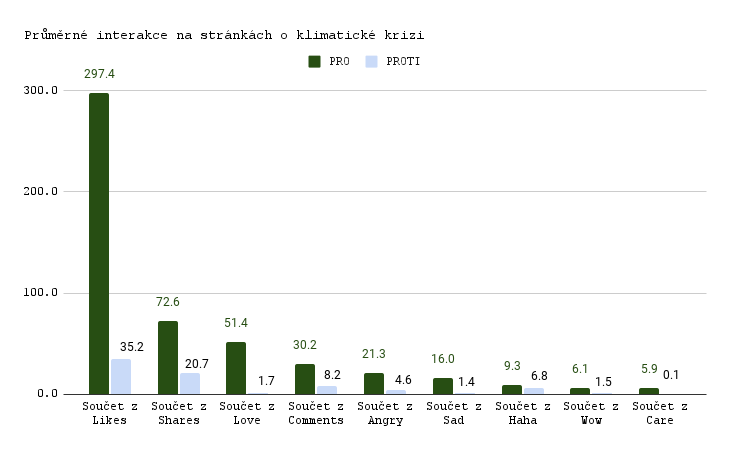
\includegraphics[width=14cm]{obrazky/Interakce na stránkách.png}
        %\centering
        %\label{fig:fb-klima-stranky-interakce}
        %\caption{Průměrné interakce na stránkách \uv{pro} i \uv{proti}. Zdroj: vlastní zpracování}
   % \end{figure}
    
    Při bližším pohledu na konkrétní interakce se ukazuje, že nejčastější reakcí (pro oba druhy stránek) jsou likes a druhou nejčastější jsou pak sdílení. Zatímco u stránek s pozitivním postojem ke klimatické změně jsou likes jednoznačně preferovanou reakcí, která tvoří více než polovinu interakcí a tvoří propast mezi dalšími reakcemi, u stránek s opačným postojem je poměr o něco málo vyváženější (ve smyslu rozdílu první a druhé nejčastější reakce) - likes tvoří okolo 40 \% interakcí a následně sdílení tvoří zaokrouhleně 26 \% z celkového počtu reakcí. Vzhledem k tomu, že u stránek \uv{pro} je poměr likes vs. sdílení 4:1 a u stránek \uv{proti} je rozdíl o trochu menší než 2:1, dá se usuzovat, že uživatelé na stránkách s negativním postojem sdílejí obsah výrazně častěji. 
    
    U stránek \uv{pro} je třetí nejčastější reakcí „love“. U stránek \uv{proti} tato interakce naopak patří mezi čtyři nejméně používané\footnote{Konkrétně šestou nejméně používanou.}. U stránek s pozitivním postojem ke klimatické změně je tedy „love“ nejsilnější reakcí, která je zároveň vyjádřením pozitivních emocí. 
    
    Na druhou stranu uživatelé, kteří konzumují obsah stránek s negativním postojem ke klimatické změně, mají větší sklon příspěvky komentovat a tento způsob interakce preferují nad jiným vyjádřením svých pocitů (prostřednictvím konkrétních reakcí „love“, „haha“, „sad“, atd.). Nejčastější emoční reakcí uživatelů na těchto stránkách je „haha“, která může být použita v různém kontextu - smích nebo ironie - přesný záměr, s jakým je použita, není jasný. 
    
    Reakce „angry“, které je výrazem negativní emoce (zloby), je u obou druhů stránek pátou nejpoužívanější reakcí. Při porovnání interakcí, které v zásadě vyjadřují negativní emoci („angry“ a „sad“) mezi stránkami \uv{pro} a \uv{proti}, se ukazuje, že uživatelé na stránkách s negativním postojem k existenci klimatické změny mají tendenci používat tuto reakci prakticky stejně často jako stránky s opačným postojem. Rozdíl v používání tvoří jen 0.2 \%. Naopak rozdíl v používání reakcí s pozitivním emočním nábojem\footnote{Myšleno reakce „love“, „wow“, „care“. „Haha“ bylo pro svůj nejasný emoční náboj vyhodnoceno jako neutrální.} je s 6.04 \% výrazně vyšší pro stránky, které mají k existenci klimatické změny pozitivní postoj.
    
    Pokud se podíváme na interakce stránek \uv{proti}, která prolomily filtrační bublinu stránek \uv{pro}, tak se všechny tři, až na Climate Change Facts, pohybují mezi prvním dvaceti stránkami s nejvyššími interakcemi. Nejsou však mezi prvními deseti. Nejúspěšnější stránky \uv{pro} v prolamování filtračních bublin na stránkách \uv{proti} jsou v počtu interakcí rozesety od 24. místa až po 200. Taktéž se tedy nejedná o stránky, které by výrazněji vyčnívaly množstvím svých interakcí nad ostatními. 

    Různé druhy obsahu mají na Facebooku rozdílný potenciál pro šíření a také pro interakce. Například textové posty/statusy mají obecně výrazně nižší interakce než například foto posty nebo videa.~\citep{newberry_mclachlan_2021} Proto bylo také sledováno, jak se liší druhy příspěvků na stránkách \uv{pro} a \uv{proti} klimatické změně. Průměrně je na stránkách \uv{proti} výrazně méně příspěvků. Zaokrouhleně 96 ku 146 na stránkách \uv{pro}. Stejně tak využití jednotlivých formátů (foto, video, status, link atd.) na stránkách \uv{proti} je ve většině případů pod průměrnými hodnotami na stránkách \uv{pro}. Jen dva druhy obsahu jsou na stránkách s negativním postojem ke klimatické změně častěji využívány než na stránkách s pozitivním postojem - textové posty/statusy, které se liší o nevýznam\-ných 0.06 příspěvků na stránku a obsah z YouTube s rozdílem 2.3. Stránky \uv{proti} sdílí v průměru méně video obsahu i fotografií a stejně jako u stránek \uv{pro} je nejčastějším druhem příspěvku link.  
    
     \begin{figure}[H]
        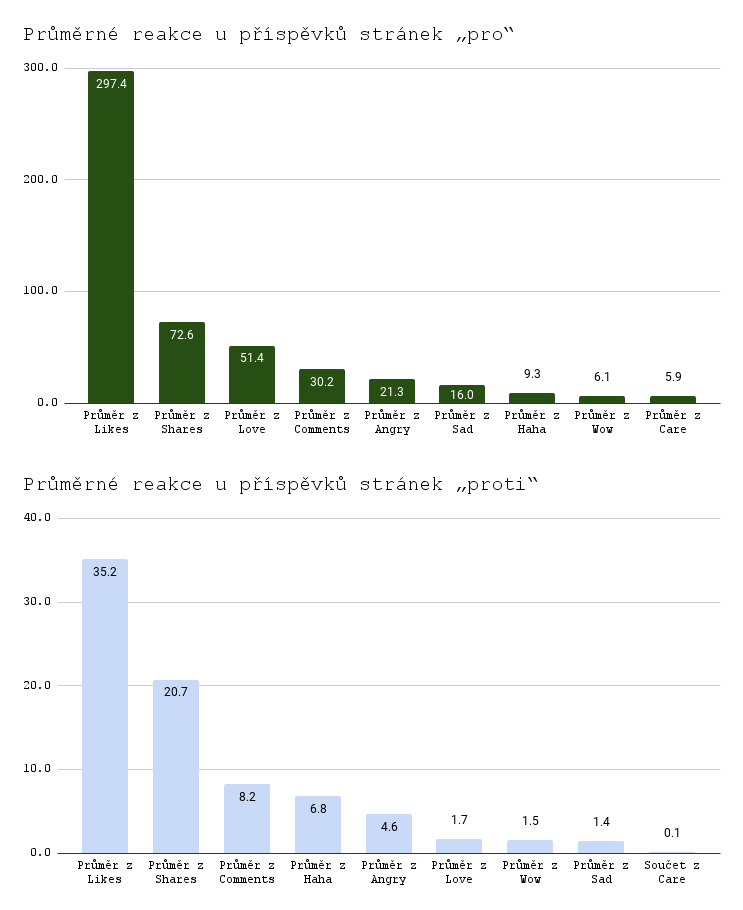
\includegraphics[width=14cm]{obrazky/Průměrné reakce u příspěvků stránek.png}
        \centering
        \caption[Průměrné interakce na stránkách \uv{pro} a \uv{proti}]{Průměrné interakce na stránkách \uv{pro} a \uv{proti} od nejvíce používaných po nejméně používané. Zdroj: vlastní zpracování}
        \label{fig:fb-klima-stranky-reakce}
    \end{figure}
\chapter{Výsledky analýzy}
\label{chapter:diskuze}
    V praktické části této práce byla uskutečněna obsahová analýza, jejímž hlav\-ním cílem bylo zjistit, zda facebookový algoritmus napomáhá prolamování informačních bublin na stránkách, které se zabývají klimatickou krizí. Na základě tohoto cíle byly následně stanoveny tři výzkumné otázky: 
    
    \begin{enumerate}
    \item Pomáhá Facebook prolamovat filtrační bubliny doporučováním stránek s různým postojem ke klimatické krizi?
    \item Jaká je frekvence doporučení stránek pro nebo proti klimatické krizi?
    \item Jak se liší interakce na doporučovaných stránkách pro a proti klimatické krizi?
    \end{enumerate}

Jak se ukázalo, facebookový algoritmus není příliš úspěšný v prolamování filtračních bublin. To je například demonstrováno na téměř nulovém prolomení bubliny u stránek, které mají pozitivní postoj k existenci klimatické změny (viz kapitola \ref{sec:prolomeni-bubliny}). Jak je možné vidět v tabulce \ref{table:prolomeni-bubliny-pro} k prolomení filtrační bubliny došlo jen u sedmi stránek \uv{pro}. Přestože u stránek s negativním postojem k existenci klimatické změny docházelo průměrně k častějšímu prolomení, na každou stránku \uv{proti} bylo doporučeno asi 1.5 stránky \uv{pro} (viz kapitola \ref{sec:prolomeni-bubliny}), nedocházelo k němu u všech stránek se stejnou mírou, ale bublina byla ve skutečnosti prolomena pouze u patnácti stránek (viz tabulka \ref{table:prolomeni-bubliny-proti}). Při takovéto míře úspěšnosti se nedá říci, že by Facebook bubliny prolamoval. Nedá se dokonce ani tvrdit, že všechny stránky o klimatické změně jsou doporučovány rovnocenně.\footnote{Interaktivní graf prolomení bublin~\ref{fig:fb-klima-stranky-bubliny}, kód, který byl využit pro stažení dat i veškerá data lze dohledat na: github.com/ryparmar/fb-related-pages}

Frekvence doporučování stránek byla celkově vyšší pro stránky s pozitivním postojem k existenci klimatické změny. V doporučení se takových stránek objevilo 540 oproti 140 stránkám s negativním postojem (viz obrázek \ref{fig:fb-klima-stranky-sireni}). To je přibližně 1 stránka \uv{proti} na 3.5 stránky \uv{pro}. To souvisí také s tím, že unikátních stránek \uv{proti} bylo v datasetu obecně méně, něž stránek \uv{pro}. Na každých 6 doporučených stránek \uv{pro} totiž připadala pouze jedna stránka \uv{proti} (viz obrázek \ref{fig:fb-klima-stranky-kategorie}). Z toho vyplývá, že stránky s negativním postojem k existenci klimatické změny se v doporučeních opakovaly mnohem častěji, než stránky s opačným postojem. Každá unikátní stránka \uv{proti} se opakovala více než 3.5x (jak je popsáno v kapitole \ref{sec:prolomeni-bubliny}). Malá skupina stránek \uv{pro} i \uv{proti} byla doporučována mnohonásobně více, oproti ostatním stránkám. Tyto stránky se nevyznačovaly žádnou společnou charakteristikou. Jednalo se o stránky různé velikosti (podle počtu fanoušků), kredibility i typu názvu. Osm nejšířenějších stránek je možné nahlédnout v tabulce \ref{fig:fb-klima-stranky-sireni}.  

Z první výzkumné otázky také vycházely stanovené hypotézy:

   \setlength\parskip{5mm}
   
    \emph{H1: Facebook doporučuje všechny stránky o klimatické změně stejnou měrou bez ohledu na jejich postoj.}
    
    \setlength\parskip{0mm}

    \emph{H2: Facebookový algoritmus posiluje vznik filtračních bublin na stránkách, které se věnují klimatické krizi.}
    
    \setlength\parskip{5mm}
   
Na základě výsledků analýzy proto můžeme říci, že hypotéza H2 byla potvrzena neboť facebookový algoritmus nebojuje úspěšně s filtračními bublinami a uživatelům nedoporučuje stránky s pozitivním a negativním postojem ke klimatické změně ekvivalentně bez ohledu na jejich postoj. 
\setlength\parskip{0mm}

Nakonec bylo v rámci provedeného výzkumu zkoumáno, jak se liší interakce na stránkách s pozitivním a s negativním postojem ke klimatické změně. Tato část analýzy (jejíž vyhodnocení je možné dohledat v kapitole \ref{sec:interakce}) byla zpracována s cílem vnést do tématiky širší kontext, který by nám mohl pomoci pochopit, zda mají interakce nějaký vliv na doporučení stránek. Bylo zjištěno, že lidé na stránkách \uv{proti} klimatické změně častěji s příspěvky interagují. Oproti stránkám \uv{pro} pak obsah více sdílejí a komentují. Naopak lidé s kladným postojem ke klimatické změně častěji používají reakce, které jsou vyjádřením nějaké pozitivní emoce. 

Nebyla ovšem zjištěna žádná přímá souvislost mezi prolomením filtrační bubliny a množstvím reakcí. Stránky s negativním postojem ke klimatické změně, které prolomily filtrační bublinu se sice pohybovaly mezi prvními dvaceti stránkami s největšími počty interakcí, ale nepatřily mezi vrchních 10 stránek. Vzhledem k celkovému počtu stránek \uv{proti} (40) navíc objektivně není tak těžké získat dobré umístění. U stránek \uv{pro}, které byly úspěšné v prolamování stránek \uv{proti} se navíc ukázalo, že se jedná o stránky, které se v počtu interakcí nachází na různých příčkách žebříčku - jak na začátku, tak i na jeho konci. 
     
%%------------------------------------------------------------------------
\section{Diskuze}
\label{sec:limity-doporuceni}
    Na první limity výzkumu narážíme ještě před prvotním sběrem dat. U doporučených stránek není jasné, podle jakých kritérií jsou stránky nabízeny. To výrazně ovlivňuje replikovatelnost celého výzkumu. Doporučení totiž nejsou stoprocentně stejná pro všechny uživatele a ještě k tomu se mění v čase. 
    
    Ke způsobu doporučování sice nebyla provedena rozsáhlá kvantitativní analý\-za, ale před začátkem výzkumu byl proveden krátký test na několika profilech, jak je uvedeno v kapitole~\ref{sec:vyber-vstup-stranek} Doporučení a výběr vstupních stránek, který ukázal výše zmíněné odlišnosti v doporučování. Seznam výsledných doporučených stránek nejvíce ovlivnil právě časový odstup, ve kterém bylo doporučeno 11 odlišných stránek oproti seznamu, který vznikl o 20 dní dříve. 
    
    Je otázkou, zda je vůbec možné na doporučení nahlížet objektivně. Může být totiž ovlivněné řadou faktorů jako například již stávajícími specifikacemi profilu, ze kterého jsou doporučení zobrazovány: seznam přátel, již zalikované stránky, předešlá aktivita apod. Pro zobrazení seznamu doporučených stránek je navíc nutné nejdříve jakoukoliv stránku liknout a i když následně její odebírání zrušíme, informace o liku a následném disliku je pravděpodobně uložena do FB databáze. Nikdy tedy nemůžeme stejnou akci na Facebooku provést za totožných podmínek. 
    
    Data byla navíc stahována během jednoho týdne a nikoli postupně, což mohlo mít samo o sobě vliv na skladbu stránek v datasetu. Jestliže se doporučení mění v čase, mohly tak být potenciálně získány lepší výsledky. Současná doporučení mohla být ovlivněna například aktuálním děním okolo klimatické změny a do seznamu se tak mohly dostat i stránky, které se běžně tomuto tématu tolik nevěnují (to platí i opačně pro případná data, která by byla sbírána později). 
    
    Dalším z limitů výzkumu, který je potřeba zmínit, je volba klíčových slov definující skóre, které bylo určující pro zařazení stránky jako klimatické. Ten byl zatížen vysokou mírou subjektivity, a to mohlo mít vliv na seznam výsledných klimaticky zaměře\-ných stránek v datasetu. Například mohlo být vybráno příliš málo slov nebo slova málo definující klimatickou změnu, což mohlo způsobit, že skóre u stránek, které se také věnují klimatické změně, nebylo dostatečně vysoké, aby prošly pomyslným sítem. 

    Při případné replikaci výzkumu je doporučeno zvolit klíčová slova jiným způso\-bem. Napří\-klad udělat seznam nejčastěji používaných slov souhrnně na všech stránkách a vybrat určitý počet těch, které se vztahují k tématu klimatické změny a zároveň patří mezi nejpoužívanější. 
    
    Je potřeba zmínit, že doporučení je pro každou stránku sice osmnáct, ale při prvním zobrazení návrhů je možné v plném rozsahu vidět pouze 4 doporučení. Pro ostatní je potřeba listovat seznamem stránek. Pokud by chtěl jednotlivec zobrazit veškeré návrhy, musí až čtyřikrát kliknout na posuvník. 
    
    To je bezpochyby určitou bariérou pro uživatele, která má pravděpodobně vliv na skutečnou schopnost stránek prolamovat filtrační bubliny. Je rozdíl mezi stránkami, které prolamují filtrační bublinu a zároveň se vyskytují hned mezi prvními čtyřmi doporučeními, a těmi, co ji sice prolamují, ale nacházejí se až na posledním listu návrhů. Domnívat se, že každý uživatel projde celý seznam doporučení a zobrazí si tak všechny stránky, by v tomto případě bylo více než optimistické. Realitě by tedy více odpovídal přístup, který by doporučeným stránkám z dostupnějších listů dával také vyšší váhu. Tento faktor nebyl v analýze zohledněn, přestože jeho promítnutí by pomohlo vylepšit kvalitu výsledků. 
    
    Nakonec je ještě třeba zmínit analýzu interakcí na doporučených stránkách, která byla provedena spíše okrajově. Jejím hlavním cílem bylo přinést do výzkumu jistý druh kontextu, který by pomohl objasnit, proč se navrhované stránky šířily uvedeným způsobem, a jaký vliv tedy mají na prolamování filtračních bublin. 
    
    Tato část výzkumu by však mohla jít mnohem více do hloubky a uvést interakce do větší souvislosti nejen s druhem obsahu (video, obrázek, sdílení atd.) šířeného na konkrétní stránce, ale mohla být také provedena lingivistická analýza názvu stránek a zveřejněného obsahu. Tento druh analýzy by mohl poodhalit nové souvislosti určující pro doporučování obsahu. Například zda stránky, které používají podobný jazyk a emoční náboj, nejsou facebookovým algoritmem identifikovány jako podobné i přes jejich opačný postoj k problematice klimatické změny. Výzkum má proto potenciál pro další bádání. 
\addcontentsline{toc}{chapter}{Závěr}
\chapter*{Závěr}
\label{chapter:zaver}
Každá společnost se musí potýkat s překážkami, které zároveň určují její další vývoj. Mezi největší současné výzvy patří klimatická změna. A přestože se o její existenci mezi odborníky diskutuje již několik let, mezi veřejností se jedná o téma, které způsobuje vysokou míru polarizace. Společnost je tak rozdělena na dva opoziční tábory, kterým se nedaří dosáhnout společného konsensu. A to i navzdory moderním informačním technologiím, které nám poskytují platformu k rovnocenné diskuzi a možnost spojit se s lidmi z celého světa. I přesto jsme od sebe navzájem v určitém smyslu mnohem izolovanější, než kdy předtím. 

Algoritmy filtrování, které nám pomáhají vyrovnat se s informačním zahlcením, jenž je tak typické pro moderní společnost, nám doporučují obsah, který je pro nás atraktivní. To nás uzavírá do filtračních bublin, kde se setkáváme stále se stejnými názory, jež nás kontinuálně utvrzují v našem již existujícím přesvědčení - což vede ještě k větší polarizaci. Naše přirozená lidská tendence tíhnout k tomu, co nám připadá správné, povědomé nebo známé pomáhá udržovat tuto propast mezi našimi a opozičními pohledy na jakoukoliv problematiku.  

To je obzvláště patrné na sociální síti Facebook, která se stala pro mnohé hlavním médiem pro komunikaci a konzumaci obsahu. Tato platforma se stala živnou půdou pro filtrační bubliny, dezinformace i fake news. Doporučovací algoritmus filtruje obsah na základě toho, co se uživatelům bude pravděpodobně líbit a s čím budou pravděpodobně interagovat. Nedokáže už však efektivně předcházet šíření obsahu, který může být pro uživatele potenciálně nebezpečný, nepravdivý a nebo porušuje zásady komunity, které si stanovuje samotný Facebook. Naopak takový obsah tento algoritmus ještě podporuje, neboť je atraktivní pro uživatele, kteří svou interakcí vyjadřují svůj zájem o tento druh příspěvku. 

Ve výzkumu, který byl uskutečněn v rámci této práce a jehož cílem bylo zjistit, zda facebookový algoritmus napomáhá prolamování filtračních bublin na facebookových stránkách, které se zabývají klimatickou změnou se ukázalo, že facebookový algoritmus selhává v účinném boji proti filtračním bublinám. Stránky, které mají pozitivní a negativní postoj ke klimatické změně v antropocentrickém pojetí, nejsou doporučovány uživatelům ekvivalentně - stránky \uv{pro} jsou oproti stránkám \uv{proti} doporučovány častěji.

Přestože častější prolamování stránek, které nesouhlasí s existencí klimatické změny (a často sdílí nepravdivý obsah) může být na jednu stranu vnímáno pozitivně, jako indicie, že se Facebook snaží zabránit šíření dezinformací (i když ne se stoprocentní úspěšností), z pohledu vzniku filtračních bublin to však až tak pozitivní znamení není. Facebookový algoritmus totiž podle všeho neumožňuje všem uživatelům dostat se k obsahu, který je vytvářen zastánci opačné ideologie, což může přispívat k zvětšování propasti mezi jednotlivými názorovými skupinami (menší toleranci a většímu vzájemnému nepochopení). To už ovšem otevírá spíše otázku etiky, svobody slova a práva na informace - neboli zda je omezování šíření fake news (nebo stránek, které je zveřejňují) služba veřejnosti nebo spíš cenzura. 

Nicméně tato práce i nadále dokazuje, že navzdory tvrzení Facebooku, je jeho fungování stále neprůhlednou černou skříňkou, která musí být podrobována dalšímu zkoumání. 

\setlength\parskip{5mm}
\begin{flushright}
   \textit{„Já ani nerozumím tomu, co myslí, když mluví o čestnosti. Myslí si, že je správné doporučovat lidem, aby se přidali k extremistickým skupinám podobným těm, které táhly na Kapitol? Jestliže všichni dostanou stejné doporučení znamená to, že je to fér?“}\footnote{Přeloženo z “I don’t even understand what they mean when they talk about fairness. Do they think it’s fair to recommend that people join extremist groups, like the ones that stormed the Capitol? If everyone gets the recommendation, does that mean it was fair?”} 
    
    - Ellery Roberts Biddle, šéfredaktor Ranking Digital Rights
    \end{flushright}
    



%%% Seznam použité literatury
%%% Seznam použité literatury (bibliografie)
%%%
%%% Pro vytváření bibliografie používáme bibTeX. Ten zpracovává
%%% citace v textu (např. makro \cite{...}) a vyhledává k nim literaturu
%%% v souboru literatura.bib.
%%%
%%% Příkaz \bibliographystyle určuje, jakým stylem budou citovány odkazy
%%% v textu. V závorce je název zvoleného souboru .bst. Styly plainnat
%%% a unsrt jsou standardní součástí latexových distribucí. Styl czplainnat
%%% je dodáván s touto šablonou a bibTeX ho hledá v aktuálním adresáři.

\bibliographystyle{czplainnat}    %% Autor (rok) s českými spojkami
% \bibliographystyle{plainnat}    %% Autor (rok) s anglickými spojkami
% \bibliographystyle{unsrt}       %% [číslo]

\renewcommand{\bibname}{Seznam použité literatury}

%%% Vytvoření seznamu literatury. Pozor, pokud jste necitovali ani jednu
%%% položku, seznam se automaticky vynechá.

\bibliography{literatura}

%%% Kdybyste chtěli bibliografii vytvářet ručně (bez bibTeXu), lze to udělat
%%% následovně. V takovém případě se řiďte normou ISO 690 a zvyklostmi v oboru.

% \begin{thebibliography}{99}
%
% \bibitem{lamport94}
%   {\sc Lamport,} Leslie.
%   \emph{\LaTeX: A Document Preparation System}.
%   2. vydání.
%   Massachusetts: Addison Wesley, 1994.
%   ISBN 0-201-52983-1.
%
% \end{thebibliography}


%%% Obrázky v diplomové práci
%%% (pokud jich je malé množství, obvykle není třeba seznam uvádět)
\listoffigures

%%% Tabulky v diplomové práci (opět nemusí být nutné uvádět)
%%% U matematických prací může být lepší přemístit seznam tabulek na začátek práce.
\listoftables

%%% Použité zkratky v diplomové práci (opět nemusí být nutné uvádět)
%%% U matematických prací může být lepší přemístit seznam zkratek na začátek práce.
% \chapwithtoc{Seznam použitých zkratek}

%%% Přílohy k diplomové práci, existují-li. Každá příloha musí být alespoň jednou
%%% odkazována z vlastního textu práce. Přílohy se číslují.
%%%
%%% Do tištěné verze se spíše hodí přílohy, které lze číst a prohlížet (dodatečné
%%% tabulky a grafy, různé textové doplňky, ukázky výstupů z počítačových programů,
%%% apod.). Do elektronické verze se hodí přílohy, které budou spíše používány
%%% v elektronické podobě než čteny (zdrojové kódy programů, datové soubory,
%%% interaktivní grafy apod.). Elektronické přílohy se nahrávají do SISu a lze
%%% je také do práce vložit na CD/DVD. Povolené formáty souborů specifikuje
%%% opatření rektora č. 72/2017.
% \appendix
% \chapter{Přílohy}

% \section{První příloha}

\openright
\end{document}
